
\documentclass[11pt]{article}

\usepackage[margin=1in]{geometry}
\usepackage[T1]{fontenc}
\usepackage{amsmath,amssymb,bm}
\usepackage{booktabs,graphicx,array}
\usepackage{float}
\usepackage{flafter}
\usepackage{amsthm}
\usepackage{newtxtext,newtxmath}
\usepackage{natbib}
\usepackage{microtype}
\usepackage{placeins}
\usepackage[hidelinks]{hyperref}

% shrink a table to the line width only when it is wider
\newcommand{\fitbox}[1]{\resizebox{\ifdim\width>\linewidth\linewidth\else\width\fi}{!}{#1}}

\renewcommand{\topfraction}{0.9}
\renewcommand{\bottomfraction}{0.8}
\renewcommand{\textfraction}{0.08}
\renewcommand{\floatpagefraction}{0.75}
\setcounter{topnumber}{3}
\setcounter{bottomnumber}{2}
\setcounter{totalnumber}{5}

\title{Measure Equivalence as a Guide for Learning SPDE Priors from Replicated Fields}
\author{Raj Jung Mahat\\[0.3em]
{\normalsize George W.\ Woodruff School of Mechanical Engineering}\\
{\normalsize Georgia Institute of Technology, Atlanta, GA 30332, USA}\\
{\normalsize \href{mailto:rajjung421@gatech.edu}{\texttt{rajjung421@gatech.edu}}}\\[0.6em]
{\small Preprint, DOI: \href{https://doi.org/10.5281/zenodo.23443597}{10.5281/zenodo.23443597}}}
\date{}

\newtheorem{proposition}{Proposition}[section]
\newtheorem{lemma}[proposition]{Lemma}
\numberwithin{table}{section}
\numberwithin{figure}{section}

\begin{document}

\maketitle

\begin{abstract}
Learning a Gaussian prior from replicated spatial fields requires deciding not only how much flexibility to add to a reference model, but where it belongs: as a correction to the reference covariance, or as a change to the differential operator that defines it. Gaussian-measure equivalence theory separates these cases in the continuum, but on any fixed discretization all nondegenerate Gaussians are equivalent, so the distinction can only be seen under mesh refinement. We study this in a leaky-aquifer SPDE where uncertain pumping, spatially varying leakage, and heterogeneous conductivity enter through the source, a lower-order term, and the principal part of the operator. Only the last changes the measure class. From 200 replicated fields whitened against a fitted reference, a diagonal refinement statistic decays to zero for source and leakage departures but stays at the plateau ($\approx0.061$) predicted for a conductivity lens. Models of the wrong class fail in characteristic ways. A stationary model absorbs source variability by driving its range to infinity ($\widehat\kappa\approx3\times10^{-5}$ against a true $\kappa_0=6$), and correction-only models fitting a conductivity change incur a KL cost that grows linearly with resolution, so reference-based complexity measures become discretization dependent. A combined model that adapts the principal operator and learns a finite-rank source correction recovers $\widehat\kappa=6.08$ on the source-only population and separates the conductivity field from the source subspace when both are present. Replicated data can therefore decide whether to correct a Gaussian reference or change its operator; deciding wrongly yields a well-fitting but structurally incorrect model.
\end{abstract}

\section{Introduction}

Gaussian random fields are widely used as probabilistic models for spatially varying quantities, and stochastic partial differential equation (SPDE) representations connect covariance structure to local differential operators \citep{Lindgren2011,LindgrenBolinRue2022}. Replicated realizations carry information about population-level covariance beyond that in a single realization, and have been used to estimate nonstationary dependence and to separate persistent population structure from realization-specific variation \citep{Ingebrigtsen2015,Fuglstad2015}. We ask whether replicated fields can reveal if a covariance discrepancy can be represented as a correction of a chosen reference model, or whether the operator defining that reference must itself change.

A common response to mismatch is to add flexibility around a reference model. One class of methods augments a simpler covariance model with low-dimensional or low-rank structure, as in fixed-rank kriging, predictive processes, and full-scale covariance approximations \citep{CressieJohannesson2008,Banerjee2008,SangHuang2012}; LatticeKrig, nearest-neighbor Gaussian processes (NNGP), and fused Gaussian processes likewise operate on the correction side of a fixed reference. A second class modifies the covariance-generating operator, for example through spatially varying range, anisotropy, or coefficients in an SPDE representation \citep{Fuglstad2015,LindgrenBolinRue2022}. Penalized-complexity (PC) priors shrink a flexible component toward a simpler base model \citep{Simpson2017,Fuglstad2019}. In each case the reference is taken as given; whether it is the right reference for the observed population is not asked.

In function space these departures are not alike: by the Feldman--H\'ajek dichotomy and the operator results of \citet{BolinKirchner2023}, smooth source and lower-order perturbations can remain in the Gaussian measure class of the reference, whereas a change of the principal coefficient cannot (Section~\ref{sec:theory}). On a finite mesh, however, all of them appear only as covariance changes.

The distinction matters for methods that learn probability measures independently of discretization. \citet{Lim2025} formulate score-based diffusion in function space under absolute-continuity and Cameron--Martin conditions relative to a Gaussian perturbing measure, and \citet{Pidstrigach2023} show that discretize-first diffusion constructions can deteriorate under mesh refinement and develop an infinite-dimensional formulation with dimension-independent guarantees. In linear inverse problems the Gaussian posterior differs from its prior only through a finite-dimensional update, and \citet{CarereLie2026} characterize low-rank posterior approximations that remain equivalent to both. Population-prior learning has no analogous guarantee that the observed population lies in the measure class of the chosen reference.

The statistical problem also differs from comparing two specified continuum models: the reference and a finite collection of replicates are observed, but the mechanism producing the discrepancy is not, and on a fixed discretization every pair of nonsingular Gaussians is mutually absolutely continuous. Fixed-domain results add a second difficulty: covariance parameters can be weakly identified while prediction remains accurate, and misspecified range parameters can produce asymptotically similar interpolation \citep{Stein1999,Zhang2004,KaufmanShaby2013}. The range parameter thus provides a weakly constrained low-frequency direction through which a stationary fit can absorb localized source variability, so a finite-resolution model can fit well while assigning variability to the wrong structural component.

Mechanism misattribution is already recognized in spatial statistics. \citet{Fuglstad2015} show that inadequately modeled mean structure can be absorbed by the covariance model, creating spurious long-range dependence or apparent nonstationarity, and replicated fields help separate competing sources of spatial variation \citep{Ingebrigtsen2015}. \citet{CuiHe2027} derive identifiability conditions for the drift and diffusion of dynamical SPDEs from trajectory data; \citet{Bolin2026} places known covariates in the forcing of an SPDE to separate pointwise and operator-mediated mean effects; and \citet{PeterssonSchroers2025} estimate and test the driving-noise covariance with the differential operator treated as given. Here the question is instead whether a covariance discrepancy across replicated equilibrium fields belongs to the source covariance or to the operator, and how the alternatives behave under mesh refinement.

The same question precedes reference-based prior construction. PC priors formalize complexity as departure from a base model \citep{Simpson2017}, parameterized for Mat\'ern fields so that the distance from the base remains meaningful \citep{Fuglstad2019}; for anisotropic SPDEs, principal-operator changes produce mutually singular measures and require alternatives to the Kullback--Leibler construction \citep{LlamazaresElias2026}. Forcing a principal-part change into a reference-based correction still gives a finite KL discrepancy on a fixed mesh, but one that grows with resolution, so the implied complexity is itself discretization dependent.

We study the question in a leaky-aquifer SPDE, where uncertain pumping, spatially varying leakage, and heterogeneous conductivity enter through the source, a lower-order term, and the principal part of the operator. The object of study is the relative covariance $T_N$ of the population with respect to the reference in reference-whitened coordinates (Section~\ref{sec:relative_covariance}), estimated from replicates by its sample counterpart $\widehat T_N$. Its spectral and refinement behavior distinguishes source-like covariance corrections from persistent principal-part discrepancy.

The resulting modeling principle is to adapt the reference operator when the population exhibits principal-part variation and to represent finite-dimensional source variability as a correction relative to the adapted reference. We implement it in a combined model that learns a spatially varying principal coefficient together with a low-rank covariance correction, each component selected separately from the data.

The contributions are fourfold. First, we use Gaussian-measure equivalence results to formulate a prior-learning problem in which source, lower-order, and principal-part departures are distinguished by their behavior under refinement, and show that a smooth principal-part departure is multiplication plus a compact operator, which fixes its refinement plateau and KL slope (Sections~\ref{sec:theory} and~\ref{sec:results_oracle}). Second, we develop a sample-based whitening and refinement diagnostic for persistent principal-part mismatch that remains informative when the departure produces no isolated eigenvalue outside the sample covariance bulk (Section~\ref{sec:results_sample}). Third, we characterize the asymmetric misattribution failures produced when source variability is represented through the operator or principal-part variability through a correction-only model, including a KL cost that grows with resolution (Section~\ref{sec:results_misattribution}). Fourth, we introduce a combined model that learns the principal operator and finite-dimensional source corrections jointly (Section~\ref{sec:results_m5}).

\section{Problem formulation and theoretical basis}
\label{sec:theory}

This section defines the population-level distinction that is later inferred from finite replicated data: what separates a covariance correction that stays in the Gaussian measure class of a reference from a departure that changes the covariance-generating operator.

\subsection{Reference field and population-learning problem}
\label{sec:reference}

Let $\mathcal D\subset\mathbb R^2$ be a bounded domain and consider the elliptic SPDE
\begin{equation}
    A_0 u = \mathcal W,
    \qquad
    A_0
    =
    \kappa_0^2 I
    -
    \nabla\!\cdot\!\left(K_0\nabla\right),
    \label{eq:reference_spde}
\end{equation}
with homogeneous Dirichlet boundary conditions. Here $\mathcal W$ denotes spatial Gaussian white noise, $\kappa_0^2$ is a zeroth-order coefficient, and $K_0$ is the principal coefficient. The nominal reference used below has $K_0\equiv1$. At the continuum level, we take $\mathcal W$ to have identity covariance in the formal white-noise coordinates. Under the present boundary conditions $A_0$ is positive and self-adjoint, so the centered reference field has law
\begin{equation}
    \mu_0
    =
    \mathcal N(0,\Sigma_0),
    \qquad
    \Sigma_0
    =
    A_0^{-1}A_0^{-1}
    =
    A_0^{-2}.
    \label{eq:reference_covariance}
\end{equation}
Equation~\eqref{eq:reference_covariance} is a continuum operator identity. Its discrete form depends on the representation of white noise. For the finite-difference scheme used in the numerical study, nodal white noise has covariance $Q_W=h^{-2}I_N$, giving $\Sigma_{0,N}=\sigma^2h^{-2}A_{0,N}^{-1}A_{0,N}^{-T}$. The complete discretization is specified in Section~\ref{sec:numerical_design}.

The value $\kappa_0=0$ remains admissible on a bounded domain with homogeneous Dirichlet conditions. In that case $A_0=-\Delta_D$, whose smallest eigenvalue is strictly positive, so the inverse and the covariance remain well defined. This observation will matter when fitting stationary reference models, because decreasing $\kappa$ corresponds to increasing the spatial range without making the bounded-domain covariance singular at $\kappa=0$.

We assume that replicated fields
\begin{equation}
    u^{(1)},\ldots,u^{(n)}
    \overset{\mathrm{iid}}{\sim}
    \mu_1
    =
    \mathcal N(0,\Sigma_1)
    \label{eq:population_replicates}
\end{equation}
are generated from an unknown population law. The prior-learning problem is to determine how $\Sigma_1$ differs structurally from the known reference covariance $\Sigma_0$. In particular, the population departure may arise through the stochastic source, through a lower-order term in the operator, or through the principal coefficient itself.

\subsection{Relative covariance in reference-whitened coordinates}
\label{sec:relative_covariance}

The comparison becomes transparent after removing the covariance already represented by the reference. Define
\begin{equation}
    T
    =
    \Sigma_0^{-1/2}
    \Sigma_1
    \Sigma_0^{-1/2}
    - I .
    \label{eq:T_continuum}
\end{equation}
If
\begin{equation}
    z=\Sigma_0^{-1/2}u,
\end{equation}
then the reference field satisfies $\operatorname{Cov}_{\mu_0}(z)=I$, while under the population law
\begin{equation}
    \operatorname{Cov}_{\mu_1}(z)=I+T.
\end{equation}
Thus $T$ is the covariance structure that remains after whitening by the reference model.

On a discretization with $N$ degrees of freedom, the corresponding matrix is
\begin{equation}
    T_N
    =
    \Sigma_{0,N}^{-1/2}
    \Sigma_{1,N}
    \Sigma_{0,N}^{-1/2}
    - I_N .
    \label{eq:T_discrete}
\end{equation}
Its eigenvalues $t_{j,N}$ quantify relative covariance departures mode by mode. The accumulated squared relative departure is
\begin{equation}
    D_N
    :=
    \|T_N\|_{\mathrm{HS}}^2
    =
    \sum_{j=1}^{N} t_{j,N}^2 .
    \label{eq:Dn}
\end{equation}
The refinement behavior of $D_N$ will provide the bridge between continuum equivalence and the finite-dimensional statistics used later.

\subsection{Gaussian equivalence and the Hilbert--Schmidt condition}
\label{sec:fh}

For two Gaussian measures on an infinite-dimensional Hilbert space, the Feldman--H\'ajek theorem gives an equivalence-or-singularity dichotomy. In one standard formulation, equivalence requires: (i) equality of the Cameron--Martin spaces, (ii) the mean difference to lie in that common space, and (iii) an appropriate relative covariance operator to be Hilbert--Schmidt \citep[Thm.~2.25]{DaPratoZabczyk2014}. All fields considered here are centered, so the mean condition is automatic. For the elliptic families below, the common-domain and Cameron--Martin conditions are supplied by the corresponding operator results; the condition that distinguishes the cases of interest is therefore the Hilbert--Schmidt behavior of the relative covariance.

Under these conditions,
\begin{equation}
    T\in\mathcal S_2
    \qquad\Longleftrightarrow\qquad
    \|T\|_{\mathrm{HS}}^2
    =
    \sum_{j=1}^{\infty}t_j^2
    <\infty ,
    \label{eq:HScriterion}
\end{equation}
where $\mathcal S_2$ denotes the Hilbert--Schmidt class. We use this condition to distinguish departures whose cumulative relative effect decays sufficiently rapidly across fine scales from departures that persist through the high-frequency spectrum.

\subsection{Three forms of population departure}
\label{sec:three_departures}

The leaky-aquifer example provides three physically distinct perturbations of \eqref{eq:reference_spde}. For each we give the operator, its measure class, and the condition that decides it.

\paragraph{Source variability.} Random pumping through $r$ smooth profiles gives
\begin{equation}
    A_0u=\mathcal W+G\xi,
    \qquad
    G\xi=\sum_{k=1}^{r}\xi_kg_k,
    \qquad
    \xi\sim\mathcal N(0,C),
    \label{eq:source_departure}
\end{equation}
so $\Sigma_1=A_0^{-1}(I+GCG^\ast)A_0^{-1}$ and, since $\Sigma_0^{1/2}=A_0^{-1}$, $T=GCG^\ast$ has rank at most $r$ and is Hilbert--Schmidt. The Cameron--Martin space of $\mu_0=\mathcal N(0,A_0^{-2})$ is $\operatorname{Ran}(A_0^{-1})$, so the induced field direction $A_0^{-1}g_k$ belongs to it exactly when $g_k\in L^2(\mathcal D)$. Smooth well profiles satisfy this condition and idealized delta sources do not, so the smooth-source assumption is load-bearing for the finite-rank in-class construction.

\paragraph{Spatially varying leakage.} Changing only the zeroth-order coefficient, $A_1=-\nabla\!\cdot(K_0\nabla)+\kappa^2(x)$, remains in the reference class in the smooth setting of \citet[Thm.~4.11 and Table~1]{BolinKirchner2023}; $T$ is Hilbert--Schmidt but generally not finite rank. With $V=\kappa^2(x)-\kappa_0^2$, to first order
\begin{equation}
    T\approx-\left(VA_0^{-1}+A_0^{-1}V\right),
    \label{eq:leakage_first_order}
\end{equation}
and for bounded smooth $V$ the singular values inherit the elliptic decay $s_j(A_0^{-1}V)=O(j^{-2/d})$, so $\sum_js_j^2\sim\sum_jj^{-4/d}$ is finite for $d<4$: infinitely many modes are affected, but with a relative effect that decays fast enough to remain Hilbert--Schmidt in $d\le3$.

\paragraph{Spatially varying conductivity.} Changing the principal coefficient, $A_1=\kappa_0^2I-\nabla\!\cdot(K_1(x)\nabla)$, leaves the class: in the variable-coefficient setting of \citet[Thm.~4.11 and Lemma~4.9]{BolinKirchner2023}, equivalence requires $K_1(x)=K_0(x)$. With the driving-noise normalization held fixed, even a constant rescaling $K_1=cK_0$, $c\neq1$, is excluded, since $(\kappa^2-c\Delta)^{-2}=c^{-2}(\kappa^2/c-\Delta)^{-2}$ changes both covariance amplitude and range.

\begin{center}
\small
\begin{tabular}{@{}llll@{}}
\toprule
Physical departure & SPDE location & Relative covariance & Model component\\
\midrule
Random smooth pumping & Source & Finite rank; in class & Low-rank correction\\
Spatially varying leakage & Zeroth order & HS; generally infinite rank ($d\le3$) & Lower-order operator\\
Spatially varying conductivity & Principal part & Outside reference class & Principal operator\\
\bottomrule
\end{tabular}
\end{center}

The variable-coefficient theorem assumes smooth coefficients and a smooth boundary. The main conductivity lens is smooth, but the unit square has corners, so we test whether the predicted refinement signature persists on the polygonal domain; a discontinuous disc lens is considered separately as a robustness experiment.

\subsection{Refinement behavior of the relative covariance}
\label{sec:refinement_criterion}

The Hilbert--Schmidt condition gives an immediate finite-resolution consequence for in-class departures.

\begin{proposition}[Bounded refinement energy for an in-class departure]
\label{prop:refinement}
Let $\{P_N\}_{N\ge1}$ be nested finite-rank orthogonal projections converging strongly to the identity, let $T\in\mathcal S_2$, and define
\begin{equation}
    T_N=P_NTP_N,
    \qquad
    D_N=\|T_N\|_{\mathrm{HS}}^2.
\end{equation}
Then
\begin{equation}
    D_N
    \longrightarrow
    \|T\|_{\mathrm{HS}}^2
    <\infty,
    \qquad
    \frac{D_N}{N}\longrightarrow0.
    \label{eq:prop_hs}
\end{equation}
\end{proposition}

The proof is given in Appendix~\ref{app:proof_refinement}. Proposition~\ref{prop:refinement} formalizes the refinement signature of an in-class departure: its accumulated squared relative covariance approaches a finite limit.

For a principal-coefficient change, \citet[Lemma~4.9]{BolinKirchner2023} establish the non-compactness that underlies failure of equivalence. Non-compactness implies that the relative perturbation does not decay in the manner required of a Hilbert--Schmidt operator, but it does not by itself imply a linear growth rate for $D_N$. The stronger scaling
\begin{equation}
    D_N=O(N),
    \qquad
    \frac{D_N}{N}\longrightarrow c>0,
    \label{eq:extensive_scaling}
\end{equation}
follows from a persistent-mode mechanism: if there exist $\rho,\delta>0$ such that at least $\rho N$ eigenvalues satisfy $|t_{j,N}|\ge\delta$, then
\begin{equation}
    D_N
    =
    \sum_{j=1}^{N}t_{j,N}^2
    \ge
    \rho N\delta^2.
    \label{eq:persistent_mode_bound}
\end{equation}
For a smooth principal-coefficient change, the following lemma shows that this mechanism is present and identifies the limits.

\begin{lemma}[A principal-part departure is multiplication plus compact]
\label{lem:mult_compact}
Let $\mathcal D\subset\mathbb R^2$ be bounded with either a smooth boundary or a convex polygonal boundary, let $K\in C^1(\overline{\mathcal D})$ with $K\ge k_0>0$, and let
\begin{equation}
    A_0=\kappa^2I-\Delta,
    \qquad
    A_1=\kappa^2I-\nabla\!\cdot(K\nabla),
\end{equation}
with the same homogeneous Dirichlet conditions and $\Sigma_j=c\,A_j^{-2}$ for a common constant $c>0$. Then
\begin{equation}
    T=\Sigma_0^{-1/2}\Sigma_1\Sigma_0^{-1/2}-I=M_m+R,
    \qquad
    m(x)=K(x)^{-2}-1,
    \label{eq:mult_compact}
\end{equation}
where $M_m$ is multiplication by $m$ and $R$ is compact on $L^2(\mathcal D)$. Consequently:
\begin{enumerate}
    \item[(i)] $\sigma_{\rm ess}(T)=m(\overline{\mathcal D})$. In particular $T$ is not compact unless $K\equiv1$.
    \item[(ii)] Let $P_N$ project onto piecewise-constant functions on a partition of $\mathcal D$ into $N$ cells of equal measure whose diameters tend to zero, and let $T_N=P_NTP_N$. Then
    \begin{equation}
        \frac{D_N}{N}\longrightarrow\frac{1}{|\mathcal D|}\int_{\mathcal D}m^2\,dx,
        \qquad
        \frac1N\sum_{i=1}^{N}(T_N)_{ii}^2\longrightarrow\frac{1}{|\mathcal D|}\int_{\mathcal D}m^2\,dx,
        \label{eq:lemma_energy}
    \end{equation}
    so the off-diagonal energy per node vanishes.
    \item[(iii)] The empirical eigenvalue distribution of $T_N$ converges weakly to the distribution of $m(X)$ with $X$ uniform on $\mathcal D$. Hence the persistent-mode condition holds with $\rho=|\{|m|\ge\delta\}|/|\mathcal D|$, and
    \begin{equation}
        \frac{\mathrm{KL}_N}{N}\longrightarrow\frac{1}{2|\mathcal D|}\int_{\mathcal D}\big[m-\log(1+m)\big]\,dx.
        \label{eq:lemma_kl}
    \end{equation}
\end{enumerate}
\end{lemma}

The proof is given in Appendix~\ref{app:proof_lemma}. Part (i) recovers the non-compactness of \citet[Lemma~4.9]{BolinKirchner2023}; parts (ii) and (iii) give the extensive scaling \eqref{eq:extensive_scaling} with an explicit constant, which equivalence theory alone does not provide. The lemma is stated for a piecewise-constant Galerkin compression; the finite-difference relative covariance used in the numerical study is a consistent approximation of it, and the agreement of the two is checked numerically in Section~\ref{sec:results_oracle}. The proof requires $K\in C^1$ and does not cover the discontinuous disc lens of Section~\ref{sec:robustness}; there the per-node energy also persists ($D_N/N\approx0.035$), which suggests that the conclusion extends, but this is not proved here.

The same distinction appears in Gaussian relative entropy. If the eigenvalues of $I+T_N$ remain bounded away from zero, then
\begin{equation}
    \mathrm{KL}_N(\mu_1\,\|\,\mu_0)
    =
    \frac12
    \sum_{j=1}^{N}
    \left[
        t_{j,N}
        -
        \log(1+t_{j,N})
    \right].
    \label{eq:gaussian_kl}
\end{equation}
For a bounded Hilbert--Schmidt perturbation this sum can converge, whereas a persistent $O(1)$ shift over a positive fraction of modes produces an $O(N)$ KL cost; for a smooth principal-coefficient change, Lemma~\ref{lem:mult_compact}(iii) gives its slope. Thus a principal-part mismatch can appear finite at every fixed discretization while becoming increasingly distant from the reference as the mesh is refined.

\subsection{What the continuum theory does not determine}
\label{sec:handoff}

These results compare known population covariances along a refinement sequence, whereas in prior learning $\Sigma_{1,N}$ is unknown and only the sample covariance $\widehat\Sigma_{1,N}=n^{-1}\sum_{i}u^{(i)}u^{(i)\top}$ of $n$ centered replicates is available, giving $\widehat T_N=\Sigma_{0,N}^{-1/2}\widehat\Sigma_{1,N}\Sigma_{0,N}^{-1/2}-I_N$. When $N/n$ is not small, sampling variability dominates: even under the exact reference, the sample covariance $S$ of $n$ draws from $\mathcal N(0,I_N)$ satisfies $\mathbb E\|S-I_N\|_F^2=N(N+1)/n$. The naive sample Hilbert--Schmidt norm therefore grows with dimension under the null and cannot serve directly as a refinement diagnostic. The continuum theory identifies \emph{what} must be distinguished but not \emph{how} to distinguish it from a finite ensemble, which is the subject of Section~\ref{sec:methods}.

\section{Statistical methodology}
\label{sec:methods}

Section~\ref{sec:theory} identifies the distinction to be inferred: bounded refinement energy for a Hilbert--Schmidt departure, against non-vanishing energy per resolved degree of freedom for a persistent principal-part departure. We first diagnose the structure of the departure from replicated fields, which must contend with finite-ensemble fluctuations, and then fit covariance models whose components can represent that structure.

\subsection{Diagnosing covariance departure from finite replicates}
\label{sec:diagnostic}

\subsubsection{Estimated reference and whitening}
\label{sec:estimated_reference}

Let
\begin{equation}
    \widehat\Sigma_{0,N}
    =
    \Sigma_{0,N}(\widehat\sigma^2,\widehat\kappa)
\end{equation}
denote the stationary reference covariance obtained by maximum likelihood from the replicated fields. We use this fitted stationary model as a \emph{reference for whitening}, not as the final covariance model. If the discrete reference covariance is written in the general form
\begin{equation}
    \Sigma_{0,N}
    =
    \sigma^2 A_\kappa^{-1}Q_W A_\kappa^{-T},
\end{equation}
with $Q_W$ the discrete white-noise covariance, a corresponding whitening map is
\begin{equation}
    z^{(j)}
    =
    \widehat\sigma^{-1}
    Q_W^{-1/2}
    A_{\widehat\kappa}u^{(j)},
    \qquad
    j=1,\ldots,n.
    \label{eq:sample_whitening}
\end{equation}
For the finite-difference discretization used in the numerical study, $Q_W=h^{-2}I$ and \eqref{eq:sample_whitening} reduces to $z=hA_{\widehat\kappa}u/\widehat\sigma$.

The whitened sample covariance is
\begin{equation}
    S
    =
    \frac1n
    \sum_{j=1}^{n}
    z^{(j)}z^{(j)\top}.
    \label{eq:whitened_sample_cov}
\end{equation}
If the reference parameters were known, $\mathbb E[S]=I+T_N$. Because the same replicated fields are used to estimate $(\widehat\sigma^2,\widehat\kappa)$, the resulting diagnostic is a plug-in statistic rather than an exactly unbiased estimate of the relative covariance. This distinction is relevant when the stationary range parameter is weakly identified or moves toward the boundary. Such range misspecification remains an in-class covariance deformation, however, and therefore cannot by itself generate a nonzero per-node refinement plateau of the type sought below. We assess the finite-sample sensitivity of the diagnostic to reference fitting separately in the numerical study.

\subsubsection{Spectral outliers and finite-dimensional source structure}
\label{sec:spectral_diag}

A finite-rank source perturbation produces isolated population eigenvalues in the whitened covariance,
\begin{equation}
    I+T
    =
    I
    +
    \sum_{k=1}^{r}c_kv_kv_k^\top,
    \qquad c_k>0 .
\end{equation}
At finite $N$ and $n$, even the null covariance produces a nontrivial sample spectrum. Let
\begin{equation}
    \gamma=\frac{N}{n}.
\end{equation}
For whitened Gaussian noise, the upper Marchenko--Pastur edge \citep{MarchenkoPastur1967} is
\begin{equation}
    \lambda_+
    =
    \left(1+\sqrt{\gamma}\right)^2 .
    \label{eq:mp_edge}
\end{equation}
We therefore report the spectral-outlier count
\begin{equation}
    \widehat r_{\mathrm{MP}}
    =
    \#\left\{
    \widehat s_k>\lambda_+
    \right\},
    \label{eq:rmp}
\end{equation}
where $\widehat s_k$ are the nonzero eigenvalues of $S$ in decreasing order. The count is used as a diagnostic for isolated positive covariance directions; the fitted correction rank is selected independently by cross-validation. A spike of strength $c_k$ separates from the bulk only above the BBP threshold $c_k>\sqrt\gamma$ \citep{BaikSilverstein2006}.

The outlier count alone cannot diagnose a principal-part departure. A spatially distributed operator change can alter many population modes without producing an isolated sample eigenvalue outside the Marchenko--Pastur bulk. This motivates a second statistic that accumulates a local signature over the spatial discretization.

\subsubsection{Diagonal refinement statistic $h_N$}
\label{sec:diag_stat}

Let
\begin{equation}
    d_i
    =
    \frac1n
    \sum_{j=1}^{n}z_{ij}^2
    \label{eq:di}
\end{equation}
denote the empirical variance of the whitened field at node $i$. For a fixed whitening reference,
\begin{equation}
    \mathbb E[d_i]
    =
    1+T_{ii}.
\end{equation}
Under Gaussian sampling,
\begin{equation}
    d_i
    \overset{d}{=}
    (1+T_{ii})\frac{\chi_n^2}{n},
\end{equation}
and therefore
\begin{align}
    \mathbb E\left[(d_i-1)^2\right]
    &=
    T_{ii}^2
    +
    \frac{2}{n}(1+T_{ii})^2,\\
    \mathbb E[d_i^2]
    &=
    \frac{n+2}{n}(1+T_{ii})^2.
\end{align}
This gives the bias-corrected statistic
\begin{equation}
    \widehat H_N
    =
    \sum_{i=1}^{N}
    \left[
        (d_i-1)^2
        -
        \frac{2}{n+2}d_i^2
    \right],
    \label{eq:Hhat}
\end{equation}
for which, conditional on a fixed whitening reference,
\begin{equation}
    \mathbb E[\widehat H_N]
    =
    \sum_{i=1}^{N}T_{ii}^2.
    \label{eq:H_unbiased}
\end{equation}
We use the normalized quantity
\begin{equation}
    \widehat h_N
    =
    \frac{\widehat H_N}{N}.
    \label{eq:hhat}
\end{equation}

The statistic is motivated by the distinction in Section~\ref{sec:theory}. If $T$ is Hilbert--Schmidt, then for any orthonormal basis
\begin{equation}
    \sum_i T_{ii}^2
    \le
    \|T\|_{\mathrm{HS}}^2
    <\infty,
\end{equation}
so the corresponding per-node diagonal energy vanishes under refinement. A principal-coefficient change has a different local high-frequency signature. By Lemma~\ref{lem:mult_compact}, the relative covariance of a smooth scalar conductivity perturbation is multiplication by
\begin{equation}
    m(x)
    =
    K(x)^{-2}-1
\end{equation}
plus a compact remainder. Consequently, under regular refinement (Lemma~\ref{lem:mult_compact}(ii)),
\begin{equation}
    \frac1N\sum_{i=1}^{N}T_{ii}^2
    \longrightarrow
    \frac{1}{|\mathcal D|}
    \int_{\mathcal D}
    \left[K(x)^{-2}-1\right]^2\,dx
    =:
    h_\infty,
    \label{eq:hlimit}
\end{equation}
for the piecewise-constant compression of the lemma; for the finite-difference grid basis used here the limit is a prediction checked against the oracle values. For the conductivity lens specified in Section~\ref{sec:numerical_design}, $h_\infty=0.060732$.

Equation~\eqref{eq:H_unbiased} is exact only when the whitening reference is fixed. Estimating the stationary reference from the same replicates introduces plug-in error, and estimating and removing source directions from the same sample introduces an additional dependence. We therefore refer to \eqref{eq:Hhat} as a bias-corrected diagnostic rather than an exactly unbiased test after fitting.

\subsubsection{Deflating isolated source directions}
\label{sec:deflation}

Mixed populations can contain both finite-dimensional source variability and a distributed principal-part departure. To expose the latter, we optionally remove isolated positive spectral directions before evaluating \eqref{eq:Hhat}. Let
\begin{equation}
    \widehat V_r
    =
    [\widehat v_1,\ldots,\widehat v_r]
\end{equation}
contain the sample eigenvectors associated with eigenvalues above the upper Marchenko--Pastur edge. The whitened fields are projected onto the orthogonal complement,
\begin{equation}
    Z_\perp
    =
    (I-\widehat V_r\widehat V_r^\top)Z.
    \label{eq:deflate_Z}
\end{equation}
Projection reduces the marginal variance at node $i$ by the leverage
\begin{equation}
    \ell_i
    =
    \sum_{k=1}^{r}\widehat v_{ik}^2.
\end{equation}
The deflated nodal variance is therefore renormalized as
\begin{equation}
    d_i^\perp
    =
    \frac{
        n^{-1}\sum_j z_{ij,\perp}^{\,2}
    }{
        1-\ell_i
    },
    \label{eq:deflated_di}
\end{equation}
and substituted into \eqref{eq:Hhat}.

In the experiments considered here, random sources add positive covariance directions while the conductivity lens is \emph{stiff}, $K(x)\ge1$, so its leading relative-covariance contribution is non-positive. Under this sign structure, upper-edge outliers provide a clean way to identify source directions before evaluating the principal-part diagnostic. For a soft lens, $K(x)<1$, a principal-part change can itself create positive high-frequency variance; the upper-edge count is then not mechanism-specific, although the diagonal refinement statistic $h_N$ remains sign-insensitive. The present deflation rule should therefore be interpreted as a source-removal step for the sign structure studied here, not as a universal classifier of all principal-part perturbations.

Because $\widehat V_r$ is estimated from the same sample used to compute $d_i^\perp$, the deflated statistic is only approximately bias corrected. A split-sample or cross-fitted implementation can remove this dependence and is used as a robustness check when evaluating the diagnostic.

\subsection{Covariance model classes}
\label{sec:model_classes}

We compare model families that place flexibility at different levels of the SPDE. All are special cases of
\begin{equation}
    \Sigma
    =
    \sigma^2
    A^{-1}
    Q_W^{1/2}
    \left(I+VCV^\top\right)
    Q_W^{1/2}
    A^{-T},
    \qquad
    V^\top V=I,
    \quad
    C=\operatorname{diag}(c_1,\ldots,c_r),\ c_k\ge0,
    \label{eq:model_family}
\end{equation}
and differ in the operator $A$ and in whether the whitened finite-rank correction $VCV^\top$ is present (Table~\ref{tab:models}). M1 is the stationary reference $A_\kappa=\kappa^2I+L$ with no correction; it defines the fitted reference used for whitening and the baseline for all comparisons. M2 keeps the eigenvectors of $L$ and reshapes the stationary modal variances by $\exp[-\delta(\lambda_j)]$, with $\delta$ a cubic B-spline expansion in $\log\lambda$, as a flexible stationary control. M3 adds the correction to the stationary base; for a fixed base, the maximum-likelihood directions are the leading eigenvectors of the whitened sample covariance, with strengths from the corresponding excess variances. M4-$\kappa$ replaces $\kappa^2$ by the spatial field $\kappa^2\exp[\Phi\theta]$, and M4-$K$ replaces $L$ by $L_{K_\theta}$ with $\log K_\theta=\Phi\theta$, where the columns of $\Phi$ are smooth radial basis functions; M4-$K$ changes the reference operator itself and is the class able to represent principal-part structure.

The combined model M5 uses both components:
\begin{equation}
    \boxed{
    \Sigma_{\mathrm{M5}}
    =
    \sigma^2
    A_\theta^{-1}
    Q_W^{1/2}
    \left(
        I+VCV^\top
    \right)
    Q_W^{1/2}
    A_\theta^{-T},
    \qquad
    A_\theta=\kappa^2I+L_{K_\theta}.
    }
    \label{eq:M5}
\end{equation}
The operator $A_\theta$ represents population variability that changes the principal spatial mechanism, while $VCV^\top$ represents finite-dimensional source variability relative to the adapted operator. M5 therefore implements the rule suggested by Section~\ref{sec:theory}: change the reference operator where the population requires a principal-part change, and represent isolated source variability as a correction around that reference.

\begin{table}[htbp]
\centering
\caption{Model classes, parameterizations and fitting protocols. Rank is selected by five-fold held-out log likelihood where applicable; numerical tolerances are listed in Table~\ref{tab:tolerances}.}
\label{tab:models}
\small
\renewcommand{\arraystretch}{1.15}
\begin{tabular}{@{}>{\raggedright\arraybackslash}p{0.08\linewidth}>{\raggedright\arraybackslash}p{0.13\linewidth}>{\raggedright\arraybackslash}p{0.19\linewidth}>{\raggedright\arraybackslash}p{0.12\linewidth}>{\raggedright\arraybackslash}p{0.17\linewidth}>{\raggedright\arraybackslash}p{0.17\linewidth}@{}}
\toprule
Model & Intended departure & Representation & Dimension / rank & Fitting & Initialization / regularization \\
\midrule
M1 &
stationary reference (baseline) &
$\sigma^2h^{-2}(\kappa^2+\lambda)^{-2}$ in the DST basis &
2 parameters &
L-BFGS-B; $\sigma^2,\kappa$ joint &
$\sigma^2=1$, $\kappa=6$; no penalty \\

M2 &
stationary misspecification (control) &
M1 $\times e^{-\delta(\lambda)}$, with six cubic B-splines in $\log\lambda$ &
8 parameters &
L-BFGS-B; joint fit &
M1 fit, $\theta=0$; no penalty \\

M3-joint &
random sources (correction) &
M1 base plus PSD spikes in whitened coordinates &
$2+r(N+1)$; $r=0,\ldots,8$ by CV &
Alternating PCA and L-BFGS-B; whitened noise fixed at 1 in PCA block &
Two starts: M1-based and $(1,\kappa_0)$; no penalty \\

M4-$\kappa$ &
leakage (lower-order operator) &
$\kappa(x)^2=\kappa^2\exp(\Phi\theta)$; 25 Gaussian RBFs &
27 parameters &
L-BFGS-B with JAX gradients; $\sigma^2$ profiled &
$\kappa=\hat\kappa_{\rm M3}$, $\theta=0$; $\lambda_\theta\|\theta\|^2$ \\

M4-$K$ &
conductivity (principal operator) &
$\log K=\Phi\theta$; same 25 RBFs &
27 parameters &
L-BFGS-B with JAX gradients; $\sigma^2$ profiled &
$\kappa=\hat\kappa_{\rm M3}$, $\theta=0$; $\lambda_\theta\|\theta\|^2$ \\

M5 &
mixed source/operator (combined) &
M4-$K$ base plus PSD whitened spikes &
$27+r(N+1)$; $r=0,\ldots,5$ by CV &
Exact block coordinate ascent: PPCA spike block and L-BFGS operator block &
Flat $K$, $\kappa=\hat\kappa_{\rm M3}$; $\lambda_\theta\|\theta\|^2$ \\
\bottomrule
\end{tabular}

\vspace{0.4em}
\footnotesize
For M3-joint, the M1-based start uses $(\hat\sigma^2_{\rm M1},\max(\hat\kappa_{\rm M1},10^{-3}))$; the second start is $(1,\kappa_0)$. The $10^{-3}$ value is an initialization floor only. For M4 and M5, $\lambda_\theta=10^{-2}$ is fixed by hand and added to the total training negative log-likelihood; held-out scores are unpenalized. RBF centres are $\{0.1,0.3,0.5,0.7,0.9\}^2$ with width $0.12$.
\end{table}

\subsection{Estimation and decision logic}
\label{sec:fitting}
\label{sec:decision_logic}

All parameters are estimated from the training replicates by likelihood or penalized likelihood, with $\sigma^2$ profiled analytically where possible. M1 and M2 are diagonal in the discrete sine-transform basis, so the likelihood is a sum over modal variances. M4-$\kappa$ and M4-$K$ minimize $-\ell(\theta,\kappa,\sigma^2)+\lambda_\theta\|\theta\|_2^2$ with $\sigma^2$ profiled out and gradients by automatic differentiation. M3 alternates between updating the whitened directions and strengths for a fixed stationary base and updating $(\sigma^2,\kappa)$ for a fixed correction; the two are alternated rather than fitted sequentially because the range parameter can absorb part of the same low-frequency variance that would otherwise appear as a source component. M5 uses exact block coordinate ascent: for fixed $(\kappa,\theta)$ the whitened spike block is updated by the PPCA closed form with a free residual variance, jointly updating $\sigma^2$, the spike directions, and their strengths, and for a fixed spike block $(\kappa,\theta)$ are updated by penalized likelihood, so each accepted update is non-decreasing in the penalized objective. M5 is initialized from a flat conductivity field rather than from the M4-$K$ solution, so that it does not inherit operator structure that M4-$K$ may have used to explain source variability. The ranks of M3 and M5 are chosen by five-fold held-out log likelihood; $\widehat r_{\mathrm{MP}}$ is reported as a diagnostic only.

The two diagnostics have complementary roles: isolated upper spectral outliers indicate finite-dimensional source structure, and a non-vanishing deflated $\widehat h_N$ indicates persistent principal-part discrepancy. Together they give the structural logic
\begin{center}
\begin{tabular}{lll}
\hline
Spectral outliers & Deflated $\widehat h_N$ & Corresponding model structure\\
\hline
present & $\to0$ & finite-rank correction (M3)\\
absent & non-vanishing & principal-operator adaptation (M4-$K$)\\
present & non-vanishing & combined adaptation and correction (M5)\\
\hline
\end{tabular}
\end{center}
This logic is evaluated, not run as an automated model-selection algorithm. A vanishing principal-part diagnostic does not by itself distinguish a stationary field from a weak lower-order perturbation; the M4-$\kappa$ comparison is retained for that purpose.

\section{Numerical study design}
\label{sec:numerical_design}

All experiments use the same reference operator and differ only in the component through which the population departs from it. We define the discretization and four synthetic populations, then the oracle refinement calculations, the finite-replicate diagnostic, and the model fits.

\subsection{Domain, discretization, and reference process}
\label{sec:design_setup}

The common setup is summarized in Table~\ref{tab:setup}; its discrete covariance is \eqref{eq:model_family} with $Q_W=h^{-2}I$. The assembled operators are symmetric, so $A^{-T}=A^{-1}$ numerically; the transpose is kept to make the construction explicit.

\begin{table}[htbp]
\centering
\caption{Common setup.}
\label{tab:setup}
\begin{tabular}{@{}ll@{}}
\toprule
Item & Value \\
\midrule
Domain & $\Omega=(0,1)^2$, $n_x\times n_x$ interior nodes, $N=n_x^2$, $h=1/(n_x+1)$ \\
Boundary condition & homogeneous Dirichlet \\
Discretisation & finite differences: 5-point stencil for $-\nabla\!\cdot(K\nabla u)$, \\
 & harmonic-mean edge conductance $2K_iK_j/(K_i+K_j)$ \\
Reference operator & $A_0=\kappa_0^2 I+L$, $\kappa_0=6$, $K_0\equiv 1$, $\sigma^2=1$ \\
White noise & $u=\sigma h^{-1}A^{-1}\xi$, $\xi\sim\mathcal N(0,I_N)$ (nodal variance $h^{-2}$) \\
Covariance & $\Sigma=\sigma^2h^{-2}A^{-1}(I+VCV^\top)A^{-T}$ \\
Whitening & $z=hAu/\sigma$ \\
Sampler & sparse LU of $A$ (direct solve) \\
Mean & zero; fields are not sample-centred \\
Fields per truth & $n_{\rm train}=200$, $n_{\rm test}=100$ \\
Seeds & main: $1000+10\,\mathrm{id}+n_x$; robustness: $+7919s$, $s=1,2,3$ \\
Sensors (held-out score) & 10 fixed points, noise s.d.\ $0.05\times$ reference RMS \\
Grids, model fits & $n_x\in\{16,32\}$ \\
Grids, diagnostics & $n_x\in\{16,24,32,48,64\}$ \\
\bottomrule
\end{tabular}
\end{table}

\subsection{Population departures}
\label{sec:design_truths}

The four populations are controlled representatives of source, lower-order, principal-part, and mixed departures (Table~\ref{tab:truths}, Figure~\ref{fig:truths}); departures are localized by the Gaussian bump $b_{c,r}(x)=\exp[-\|x-c\|^2/2r^2]$. Truth A is constructed directly in reference-whitened coordinates from three unit-norm Gaussian directions, so the population is exactly of the M3 form; the smooth nodal directions discretize admissible $L^2$ source profiles, not point sources. Truth B$'$ changes only the zeroth-order term, with a smooth leakage dip toward the lens centre. Truth B changes the principal coefficient through
\begin{equation}
    K(x)=\exp\!\left[b_{c_L,r_L}(x)\right],
    \label{eq:truthB_K}
\end{equation}
which varies smoothly from $1$ to $e$, so the remaining mismatch with the operator theorem is the square's nonsmooth boundary. Truth C composes exactly the B operator with exactly the A spike directions and strengths, without retuning either.

\begin{table}[htbp]
\centering
\caption{The truths. $b_{c,r}(x)=\exp(-\|x-c\|^2/2r^2)$; $v_k=b_{c_k,r_w}/\|b_{c_k,r_w}\|_2$ (nodal norm).}
\label{tab:truths}
\begin{tabular}{@{}llll@{}}
\toprule
Truth & Operator $A$ & Spikes $VCV^\top$ & Parameters \\
\midrule
ref & $\kappa_0^2I+L$ & --- & $\kappa_0=6$ \\
A (wells) & $\kappa_0^2I+L$ & $\sum_k c_k v_kv_k^\top$ & centres $(0.25,0.30)$, $(0.70,0.25)$, $(0.55,0.75)$; \\
 & & & $r_w=0.05$; $c=(90,60,40)$ \\
B$'$ (leakage) & $\mathrm{diag}(\kappa(x)^2)+L$ & --- & $\kappa(x)^2=\kappa_0^2+\gamma\,b_{c_L,r_L}$, $\gamma=-30$ \\
 & & & ($\kappa^2$ from 36 to 6 at the centre) \\
B (lens) & $\kappa_0^2I+L_K$ & --- & $K=\exp(\beta\,b_{c_L,r_L})$, $\beta=1$: smooth, $K\in[1,e]$ \\
C (wells+lens) & $\kappa_0^2I+L_K$ & as A & as A and B \\
\midrule
\multicolumn{4}{@{}l}{Lens and leakage: $c_L=(0.5,0.5)$, $r_L=0.12$; off-grid robustness lens $c_L=(0.42,0.57)$.} \\
\multicolumn{4}{@{}l}{Robustness of the oracle diagnostic only: disc lens $K=e\,\mathbb 1_{\|x-c_L\|\le 0.12}+\mathbb 1_{\rm else}$; constant $K\equiv1.5$.} \\
\bottomrule
\end{tabular}
\end{table}

\begin{figure}[htbp]
    \centering
    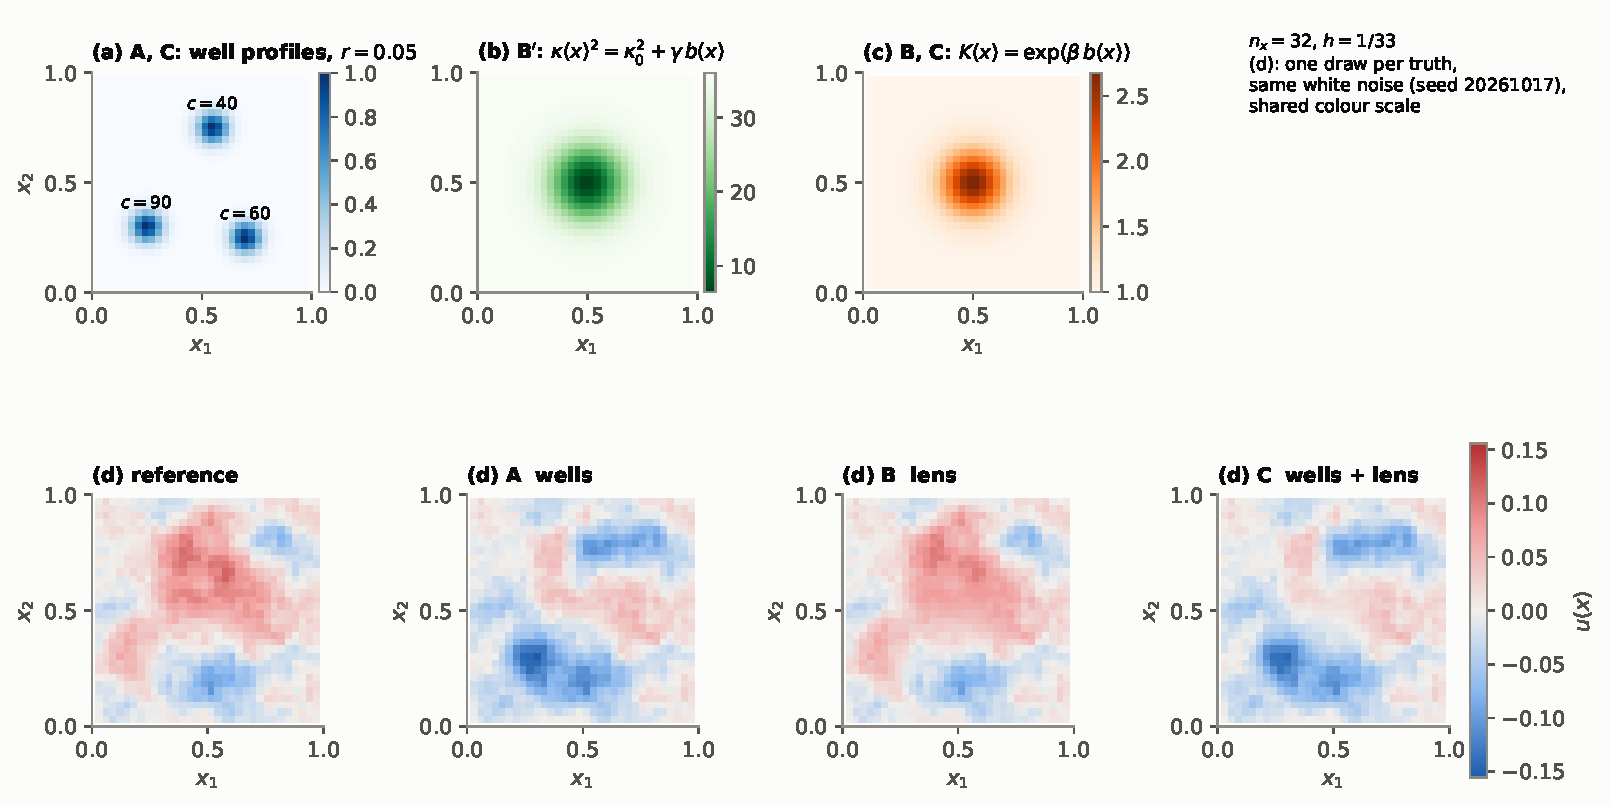
\includegraphics[width=\linewidth]{figures/fig4_1_truths.pdf}
    \caption{Synthetic population construction at $n_x=32$. The top row shows the three normalized well profiles used in A and C, the spatially varying leakage coefficient used in B$'$, and the smooth conductivity field used in B and C. The bottom row shows one draw from the reference, A, B, and C generated with the same white-noise realization and displayed on a common colour scale.}
    \label{fig:truths}
\end{figure}

\subsection{Replicates and resolution regimes}
\label{sec:design_regimes}

Each main fit uses $n_{\rm train}=200$ independent zero-mean training fields and $n_{\rm test}=100$ test fields. Model fitting uses $n_x\in\{16,32\}$ and the refinement diagnostic $n_x\in\{16,24,32,48,64\}$, so at fixed ensemble size the aspect ratio $\gamma=N/n_{\rm train}$ grows along the refinement sequence (Table~\ref{tab:regimes}) and the diagnostic is tested in an increasingly high-dimensional regime. The well width is below one mesh spacing at $n_x=16$, so refinement also changes the spatial resolution of the source profiles: spike strengths at $n_x=16$ are not comparable discretizations of the finer-grid amplitudes, and the decay of source-only statistics starts from an under-resolved representation. The sample-based refinement experiment uses five independently generated training ensembles of 200 fields per truth and resolution; additional seeds are reserved for robustness checks.

\begin{table}[htbp]
\centering
\caption{Regimes per grid ($n_{\rm train}=200$). $\sqrt\gamma$ is the BBP detection threshold for a
whitened spike; features are resolved by $r/h$ cells.}
\label{tab:regimes}
\begin{tabular}{@{}rrrrrrr@{}}
\toprule
$n_x$ & $N$ & $\gamma=N/n_{\rm train}$ & $\sqrt\gamma$ & MP edge $(1+\sqrt\gamma)^2$ & $r_w/h$ & $r_L/h$ \\
\midrule
16 & 256  & 1.28  & 1.131 & 4.543  & 0.85 & 2.04 \\
24 & 576  & 2.88  & 1.697 & 7.274  & 1.25 & 3.00 \\
32 & 1024 & 5.12  & 2.263 & 10.645 & 1.65 & 3.96 \\
48 & 2304 & 11.52 & 3.394 & 19.308 & 2.45 & 5.88 \\
64 & 4096 & 20.48 & 4.525 & 30.531 & 3.25 & 7.80 \\
\bottomrule
\end{tabular}
\end{table}

\subsection{Oracle refinement quantities and predictions}
\label{sec:oracle_design}

Because the population covariance is known, the first experiment evaluates $T_N$ directly, without sampling error, and records the relative spectrum, $D_N=\|T_N\|_F^2$, $D_N/N$, $\mathrm{KL}_N(\mu_1\|\mu_0)$, and the diagonal energy
\begin{equation}
    h_N^{\rm oracle}
    =
    \frac1N\sum_{i=1}^{N}T_{ii}^2,
    \label{eq:oracle_hN_design}
\end{equation}
which is the population target of $\widehat h_N$. For the smooth lens, midpoint quadrature of \eqref{eq:hlimit} from $256^2$ through $2048^2$ points agrees with $h_\infty=0.060732$ at the reported precision. The finite-grid oracle values approach $h_\infty$ from above and remain about $2.5\%$ above it at $n_x=64$ (Table~\ref{tab:T5_1}), so $\widehat h_N$ is compared with $h_N^{\rm oracle}$ at each grid and $h_\infty$ serves only as the asymptotic target. These quantities depend only on the configured truth and reference and were computed before any sample-based fitting.

\subsection{Sample diagnostic protocol}
\label{sec:sample_protocol}

At each truth and resolution, M1 is fitted to the 200 training fields and used as the plug-in whitening reference. Positive isolated directions are counted with the unmodified edge \eqref{eq:mp_edge} at $\gamma=N/n_{\rm train}$, i.e.\ multiplicative edge factor $1.0$ with no finite-sample safety margin, so an isolated eigenvalue can occasionally cross it under the reference and the count is a diagnostic rather than a level-controlled test. The leverage correction \eqref{eq:deflated_di} uses a denominator floor of $10^{-3}$, and the variance term in \eqref{eq:Hhat} uses the actual number of fields in the evaluated ensemble. $\widehat h_N$ is reported with and without positive-spike deflation and compared with \eqref{eq:oracle_hN_design}. Because the reference and deflation directions are estimated from the data, a cross-fitted analysis estimates them on one subset of fields and evaluates $\widehat h_N$ on an independent subset.

\subsection{Model-fitting protocol}
\label{sec:model_fit_design}

All models in Table~\ref{tab:models} are fitted to the same training ensembles. M1 is initialized at the reference values and optimized without bounds on $\kappa$. M4-$\kappa$, M4-$K$ and M5 share the 25 radial basis functions and the penalty weight $\lambda_\theta=0.01$ listed under Table~\ref{tab:models}; the weight is fixed by hand rather than by cross-validation, and because the likelihood scales with both the number of fields and the field dimension it is small relative to the data term. The M3 PCA step fixes the whitened baseline noise variance at one, whereas the M5 PPCA step leaves it free; the M5 cycle stops on a per-cycle objective tolerance.

\subsection{Evaluation metrics}
\label{sec:evaluation_metrics}

Models are scored on the same 100 held-out fields per truth. The primary score is the full-field Gaussian log likelihood relative to the generating model on the same fields,
\begin{equation}
    \Delta\ell
    =
    \frac{1}{n_{\rm test}}\sum_{i=1}^{n_{\rm test}}
    \left[\log p_{\widehat\Sigma}(u_i)-\log p_{\Sigma_1}(u_i)\right]
    \qquad\text{(nats per field; $0$ = truth).}
\end{equation}
The secondary score conditions on ten noisy point observations,
\begin{equation}
    y=Hu+\varepsilon,
    \qquad
    \varepsilon\sim\mathcal N(0,\sigma_y^2I),
\end{equation}
with $\sigma_y$ equal to $5\%$ of the reference-field RMS, and records the conditional log predictive density of the full field, $\log p(u_{\rm test}\mid y)$, and the RMSE of the Gaussian posterior mean; it tests whether a learned prior stays useful under sparse observations. Mechanism recovery is assessed separately: $\mathrm{corr}(\log\widehat K,\log K_{\rm true})$ and $\widehat\kappa$ on B and C, and the selected rank, spike strengths, per-direction cosines, and principal-angle cosines to the true source subspace on A and C.

\subsection{Robustness analyses and chronology}
\label{sec:robustness_design}

The robustness analyses of Section~\ref{sec:robustness} repeat the model comparison on three fresh seeds and with the lens moved off the RBF grid, repeat the oracle calculation for a disc lens and for constant $K\equiv1.5$, vary $\lambda_\theta$ and the B$'$ replicate count, cross-fit the sample diagnostic, and compare the exact M5 fit used throughout with an earlier legacy update.

The sequence of analyses is recorded explicitly. The physical departures and the oracle refinement predictions were specified before the sample-based statistic $\widehat h_N$ and M5 were developed. Those two, and the explicit wrong-operator check of M4-$K$ on the source-only truth A, were introduced afterward to address the finite-ensemble classification problem and the mixed source/operator population, and are evaluated separately from the oracle calculations.

\section{Results: refinement behavior and mechanism attribution}
\label{sec:results}

The results address four questions: whether refinement recovers the continuum distinction when the population covariance is known exactly, whether the distinction survives estimation from 200 replicated fields, what happens when a departure is forced into the wrong structural component, and whether the combined model uses its two components selectively. The emphasis is on mechanism attribution rather than on predictive ranking alone.

\subsection{Oracle refinement separates finite-rank, lower-order, and principal-part departures}
\label{sec:results_oracle}

Table~\ref{tab:T5_1} compares the exact relative covariance under refinement. Truth A is defined directly in whitened coordinates, so $T_N=VCV^\top$ exactly at every grid, and $D_N=\sum_kc_k^2=13300$ and $\mathrm{KL}_N=\tfrac12\sum_k[c_k-\log(1+c_k)]=88.83$ hold by construction; these rows check the computation rather than test the theory, and $D_N/N$ falls as $N$ grows. The in-class evidence comes from the leakage perturbation B$'$, whose relative covariance is neither finite rank nor fixed by construction: $D_N$ and $\mathrm{KL}_N$ approach finite limits while $D_N/N$ and $h_N$ tend to zero, as expected of an infinite-rank but Hilbert--Schmidt departure.

The conductivity lens B is extensive: $D_N/N$ is nearly constant over the five grids, and a least-squares line gives $\mathrm{KL}_N\approx0.16+0.0315N$ with log--log slope $1.001$. Table~\ref{tab:T5_1} also checks the two quantitative predictions of Lemma~\ref{lem:mult_compact}. First, the gap between $D_N/N$ and $h_N$ shrinks from $8.3\times10^{-4}$ to $6\times10^{-5}$ over the five grids (from $1.3\%$ to $0.1\%$ of $h_N$), so the off-diagonal relative covariance energy per node vanishes, as it must for multiplication plus a compact remainder, and $h_N$ approaches $h_\infty$ from above. Second, the lemma predicts the KL slope
\begin{equation}
    \frac{1}{2|\mathcal D|}\int_{\mathcal D}\big[m-\log(1+m)\big]\,dx=0.030796
\end{equation}
for the lens; the exact $\mathrm{KL}_N/N$ lie $2$--$3\%$ above it, the same relative offset as $h_N$ above $h_\infty$ at $n_x=64$, so the fitted slope is a prediction rather than a fit. The smooth conductivity perturbation therefore realizes the persistent-mode behavior of Section~\ref{sec:refinement_criterion} rather than merely violating equivalence abstractly.

The $L^2$-Wasserstein distance gives a contrast: for B it stays near $4\times10^{-3}$ while $\mathrm{KL}_N$ grows linearly, so the fields remain close in an ordinary transport metric while their covariance ratio accumulates an extensive high-frequency discrepancy. Truth C superposes the two mechanisms: at the available resolutions $D_N/N$ is dominated by the finite-rank source component and decreases, while $\mathrm{KL}_N$ grows and $h_N$ approaches the lens contribution from above, so the different summaries separate the finite-dimensional and distributed parts of the mixed departure.

\begin{table}[htbp]
\centering
\caption{Oracle refinement. $D_N=\|T\|_{\rm HS}^2$, $\mathrm{KL}_N=\mathrm{KL}(\mu_1\|\mu_0)$, $h_N=\frac1N\sum_iT_{ii}^2$, $W_2$ in $L^2(\Omega)$ units. Lens limit $h_\infty=0.060732$.}
\label{tab:T5_1}
\begin{tabular}{@{}llrrrrrr@{}}
\toprule
Truth & $n_x$ & $N$ & $D_N$ & $D_N/N$ & $\mathrm{KL}_N$ & $h_N$ & $W_2$ \\
\midrule
A & 16 & 256 & 13300.00 & 51.9531 & 88.83 & 11.83470 & 0.0754 \\
 & 24 & 576 & 13300.00 & 23.0903 & 88.83 & 2.35010 & 0.0748 \\
 & 32 & 1024 & 13300.00 & 12.9883 & 88.83 & 0.75929 & 0.0746 \\
 & 48 & 2304 & 13300.00 & 5.7726 & 88.83 & 0.15306 & 0.0745 \\
 & 64 & 4096 & 13300.00 & 3.2471 & 88.83 & 0.04893 & 0.0744 \\
\midrule
B$'$ & 16 & 256 & 0.61 & 0.0024 & 0.11 & 0.00058 & 0.0040 \\
 & 24 & 576 & 0.60 & 0.0010 & 0.11 & 0.00015 & 0.0040 \\
 & 32 & 1024 & 0.59 & 0.0006 & 0.11 & 0.00006 & 0.0040 \\
 & 48 & 2304 & 0.59 & 0.0003 & 0.11 & 0.00001 & 0.0040 \\
 & 64 & 4096 & 0.59 & 0.0001 & 0.11 & $4.97\times10^{-6}$ & 0.0040 \\
\midrule
B & 16 & 256 & 16.54 & 0.0646 & 8.03 & 0.06380 & 0.0043 \\
 & 24 & 576 & 36.88 & 0.0640 & 18.30 & 0.06363 & 0.0042 \\
 & 32 & 1024 & 65.01 & 0.0635 & 32.54 & 0.06325 & 0.0042 \\
 & 48 & 2304 & 144.61 & 0.0628 & 72.88 & 0.06266 & 0.0041 \\
 & 64 & 4096 & 255.33 & 0.0623 & 129.01 & 0.06228 & 0.0041 \\
\midrule
C & 16 & 256 & 11099.86 & 43.3588 & 87.61 & 10.22121 & 0.0707 \\
 & 24 & 576 & 11149.76 & 19.3572 & 98.00 & 2.02637 & 0.0701 \\
 & 32 & 1024 & 11193.69 & 10.9313 & 112.30 & 0.68665 & 0.0699 \\
 & 48 & 2304 & 11285.31 & 4.8981 & 152.69 & 0.18169 & 0.0697 \\
 & 64 & 4096 & 11400.42 & 2.7833 & 208.84 & 0.09730 & 0.0697 \\
\bottomrule
\multicolumn{8}{@{}p{0.97\linewidth}}{\footnotesize $W_2$ at $n_x=24,48$ computed for this table with the same routine as the stored values (\texttt{run\_robust\_T.w2}; it reproduces the stored $n_x=16$ values to $10^{-15}$). The reference is identically zero at every grid and is omitted.} \\
\end{tabular}
\end{table}

\subsection{The refinement distinction survives finite sampling}
\label{sec:results_sample}

The sample experiment replaces the population covariance by 200 replicated fields whitened with a fitted stationary M1 (Figure~\ref{fig:F5_2}, Table~\ref{tab:T5_2}). The two-scale diagnostic retains the oracle distinction despite both finite-sample covariance noise and reference fitting.

Under the reference population, $\widehat h_N$ fluctuates around zero at all resolutions; the unmodified Marchenko--Pastur edge occasionally admits one apparent upper outlier, consistent with the role of $\widehat r_{\rm MP}$ as a diagnostic rather than a level-controlled test (Section~\ref{sec:sample_protocol}). On A, exactly three upper outliers are detected in every replicate at every resolution; the raw statistic is dominated by the localized source directions, and after deflation $\widehat h_N$ tends toward zero. This holds even though the stationary whitening fit drives $\widehat\kappa$ toward the boundary: a plug-in reference badly distorted in its low-frequency range parameter does not produce a persistent fine-scale diagonal plateau. The weak leakage case B$'$ gives no stable outlier count, and both raw and deflated $\widehat h_N$ fluctuate around zero at the finer grids.

B instead remains nearly resolution invariant and close to the finite-grid oracle targets. For the stiff lens $K\ge1$ the leading principal-part contribution to the lens block of $T$ is non-positive, so the positive directions deflated on B are occasional finite-sample upper-edge crossings rather than lens signal. Removing them lowers the in-sample estimate by $0.0004$--$0.0015$, to within $1\%$ of $h_\infty$, but part of that agreement is a same-sample selection effect: with cross-fitted deflation (Table~\ref{tab:r-crossfit}) the deflated and raw values on B coincide, at $0.4$--$3.2\%$ above $h_\infty$ and $1.5$--$2.7\%$ below the finite-grid oracle. The plateau, not its third digit, is the finding. The persistent principal-part signature is therefore visible from replicated fields without access to $\Sigma_1$.

The mixed truth C is the more stringent test, because the fitted stationary reference again collapses its range and the raw statistic is dominated by three source directions. These are recovered as upper outliers in every replicate, and after their removal $\widehat h_N$ approaches the lens-scale plateau seen under B rather than tending to zero as under A: deflation exposes the distributed principal-part component beneath the finite-dimensional spikes. Because the deflation directions are estimated from the same fields, the absolute values are a bias-corrected diagnostic rather than an exactly unbiased estimate; the refinement pattern is the principal result.

\begin{figure}[htbp]
    \centering
    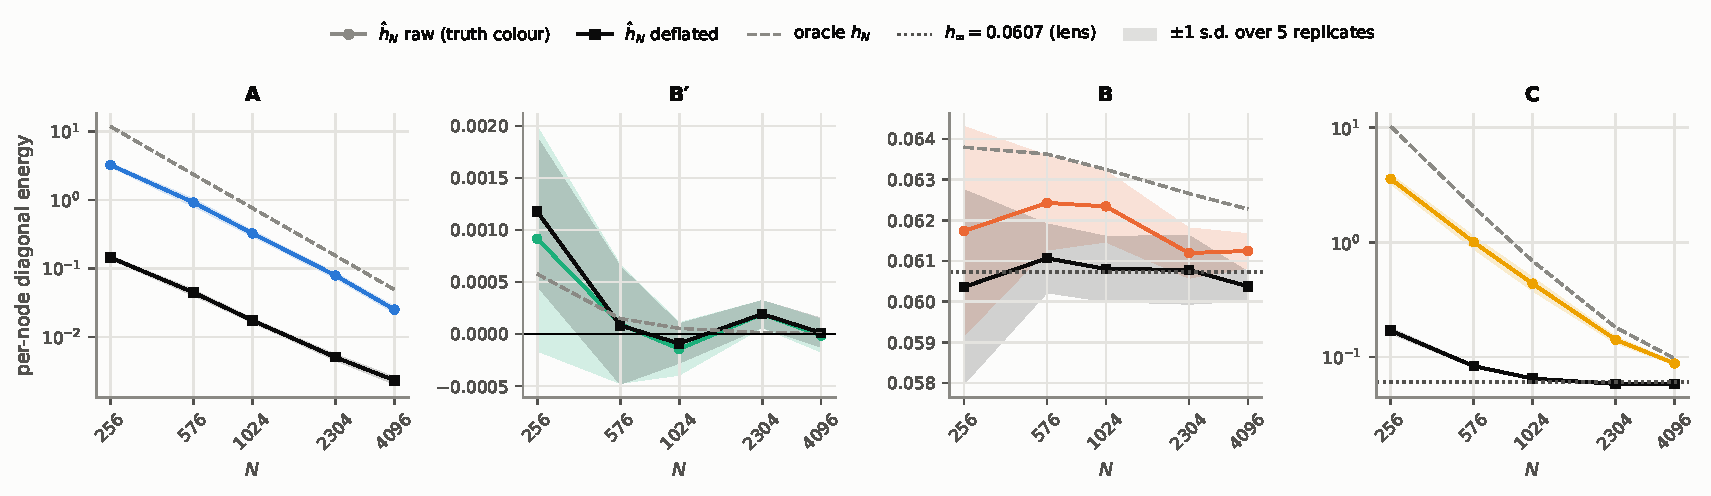
\includegraphics[width=\linewidth]{figures/fig5_2_sample_vs_oracle.pdf}
    \caption{Diagonal refinement statistic $\widehat h_N$ from 200 fields whitened by a fitted M1, raw (truth colour) and after deflating the eigenvalues above the Marchenko--Pastur edge (black); bands show $\pm1$ standard deviation over five replicates. Dashed curves show the oracle $h_N$. Dotted curves for B and C show $h_\infty=0.0607$. On A and B$'$ the deflated statistic decreases under refinement; on B and C it remains at the lens scale.}
    \label{fig:F5_2}
\end{figure}

\begin{table}[htbp]
\centering
\caption{Diagonal refinement statistic from 200 training fields, whitened by a fitted M1 (5 replicates, mean $\pm$ s.d.). $r_{\rm MP}$: eigenvalues above $(1+\sqrt{N/200})^2$ (edge factor 1.0); $\hat h_N=\hat H/N$ before and after deflating those $r_{\rm MP}$ directions.}
\label{tab:T5_2}
\fitbox{%
\begin{tabular}{@{}llrrrrr@{}}
\toprule
Truth & $n_x$ & $r_{\rm MP}$ & $\hat\kappa$ & $\hat\sigma^2$ & $\hat h_N$ raw & $\hat h_N$ deflated \\
\midrule
ref & 16 & 0.0 $\pm$ 0.0 & 6.04 $\pm$ 0.19 & 1.003 $\pm$ 0.006 & 0.0002 $\pm$ 0.0004 & 0.0002 $\pm$ 0.0004 \\
 & 24 & 0.0 $\pm$ 0.0 & 5.98 $\pm$ 0.15 & 1.000 $\pm$ 0.005 & -0.0003 $\pm$ 0.0004 & -0.0003 $\pm$ 0.0004 \\
 & 32 & 0.2 $\pm$ 0.4 & 6.01 $\pm$ 0.08 & 1.000 $\pm$ 0.002 & 0.0001 $\pm$ 0.0004 & 0.0001 $\pm$ 0.0004 \\
 & 48 & 0.2 $\pm$ 0.4 & 6.10 $\pm$ 0.10 & 1.000 $\pm$ 0.002 & 0.0001 $\pm$ 0.0004 & 0.0002 $\pm$ 0.0004 \\
 & 64 & 0.0 $\pm$ 0.0 & 6.00 $\pm$ 0.07 & 1.001 $\pm$ 0.001 & $-2.93\times10^{-5}$ $\pm$ 0.0002 & $-2.93\times10^{-5}$ $\pm$ 0.0002 \\
\midrule
A & 16 & 3.0 $\pm$ 0.0 & $0.00163\pm0.00193$ & 1.437 $\pm$ 0.032 & 3.2405 $\pm$ 0.2088 & 0.1440 $\pm$ 0.0092 \\
 & 24 & 3.0 $\pm$ 0.0 & $(1.52\pm1.08)\times10^{-4}$ & 1.186 $\pm$ 0.017 & 0.9177 $\pm$ 0.1201 & 0.0445 $\pm$ 0.0046 \\
 & 32 & 3.0 $\pm$ 0.0 & $(8.34\pm6.30)\times10^{-5}$ & 1.098 $\pm$ 0.007 & 0.3239 $\pm$ 0.0322 & 0.0173 $\pm$ 0.0013 \\
 & 48 & 3.0 $\pm$ 0.0 & $(1.33\pm0.83)\times10^{-4}$ & 1.041 $\pm$ 0.003 & 0.0789 $\pm$ 0.0077 & 0.0050 $\pm$ 0.0005 \\
 & 64 & 3.0 $\pm$ 0.0 & $(2.01\pm0.69)\times10^{-4}$ & 1.023 $\pm$ 0.002 & 0.0250 $\pm$ 0.0028 & 0.0023 $\pm$ 0.0003 \\
\midrule
B$'$ & 16 & 0.6 $\pm$ 0.8 & 5.45 $\pm$ 0.16 & 0.993 $\pm$ 0.009 & 0.0009 $\pm$ 0.0011 & 0.0012 $\pm$ 0.0007 \\
 & 24 & 0.2 $\pm$ 0.4 & 5.47 $\pm$ 0.12 & 1.000 $\pm$ 0.003 & $9.65\times10^{-5}$ $\pm$ 0.0006 & $8.36\times10^{-5}$ $\pm$ 0.0006 \\
 & 32 & 0.2 $\pm$ 0.4 & 5.49 $\pm$ 0.15 & 0.997 $\pm$ 0.005 & -0.0001 $\pm$ 0.0003 & $-9.02\times10^{-5}$ $\pm$ 0.0002 \\
 & 48 & 0.0 $\pm$ 0.0 & 5.59 $\pm$ 0.11 & 0.999 $\pm$ 0.002 & 0.0002 $\pm$ 0.0001 & 0.0002 $\pm$ 0.0001 \\
 & 64 & 0.2 $\pm$ 0.4 & 5.52 $\pm$ 0.08 & 0.999 $\pm$ 0.001 & $-1.36\times10^{-5}$ $\pm$ 0.0002 & $1.27\times10^{-5}$ $\pm$ 0.0001 \\
\midrule
B & 16 & 0.6 $\pm$ 0.5 & 5.96 $\pm$ 0.15 & 0.864 $\pm$ 0.005 & 0.0617 $\pm$ 0.0026 & 0.0604 $\pm$ 0.0024 \\
 & 24 & 0.8 $\pm$ 0.4 & 6.04 $\pm$ 0.17 & 0.874 $\pm$ 0.003 & 0.0624 $\pm$ 0.0012 & 0.0611 $\pm$ 0.0008 \\
 & 32 & 1.2 $\pm$ 0.4 & 5.94 $\pm$ 0.09 & 0.871 $\pm$ 0.003 & 0.0623 $\pm$ 0.0009 & 0.0608 $\pm$ 0.0008 \\
 & 48 & 0.4 $\pm$ 0.5 & 6.01 $\pm$ 0.12 & 0.875 $\pm$ 0.003 & 0.0612 $\pm$ 0.0006 & 0.0608 $\pm$ 0.0008 \\
 & 64 & 1.0 $\pm$ 0.6 & 6.06 $\pm$ 0.09 & 0.876 $\pm$ 0.001 & 0.0612 $\pm$ 0.0004 & 0.0604 $\pm$ 0.0004 \\
\midrule
C & 16 & 3.0 $\pm$ 0.0 & $(0.741\pm1.247)\times10^{-3}$ & 1.254 $\pm$ 0.029 & 3.5717 $\pm$ 0.3379 & 0.1702 $\pm$ 0.0100 \\
 & 24 & 3.0 $\pm$ 0.0 & $0.00442\pm0.00359$ & 1.034 $\pm$ 0.013 & 1.0032 $\pm$ 0.1295 & 0.0835 $\pm$ 0.0026 \\
 & 32 & 3.0 $\pm$ 0.0 & $(8.16\pm5.11)\times10^{-5}$ & 0.964 $\pm$ 0.010 & 0.4367 $\pm$ 0.0596 & 0.0651 $\pm$ 0.0017 \\
 & 48 & 3.0 $\pm$ 0.0 & $0.00331\pm0.00401$ & 0.915 $\pm$ 0.003 & 0.1418 $\pm$ 0.0097 & 0.0585 $\pm$ 0.0004 \\
 & 64 & 3.0 $\pm$ 0.0 & $0.00158\pm0.00291$ & 0.898 $\pm$ 0.002 & 0.0881 $\pm$ 0.0030 & 0.0582 $\pm$ 0.0001 \\
\bottomrule
\multicolumn{7}{@{}p{0.97\linewidth}}{\footnotesize Entries are mean $\pm$ s.d. over five replicate ensembles. On A and C the M1 $\hat\kappa$ collapses to $10^{-5}$--$10^{-2}$; scientific notation is used where needed to retain the spread.} \\
\end{tabular}}
\end{table}

\subsection{Wrong-class models fit by reallocating variability to the wrong mechanism}
\label{sec:results_misattribution}

When a model class cannot represent the true mechanism directly, the question is which of its available components absorbs the discrepancy. Figure~\ref{fig:F5_3} and Tables~\ref{tab:T5_3}--\ref{tab:T5_4b} show that the resulting failures are systematic rather than simple losses in predictive score.

On the source-only truth A, the stationary model absorbs the low-frequency effect of the wells by driving its range parameter to the boundary, with $\widehat\kappa$ of order $10^{-5}$ against the generating $\kappa_0=6$ (Table~\ref{tab:T5_4}). M2 improves held-out likelihood with a flexible stationary spectrum but follows the same collapsed range. M4-$K$ misattributes differently, placing conductivity structure around the wells while again collapsing $\widehat\kappa$ (Figure~\ref{fig:F5_3}a, Table~\ref{tab:T5_3}). Joint source correction resolves both failures: M3-joint selects rank three and returns $\widehat\kappa$ close to $6$. M3-nested, which fits the stationary reference first and adds spikes afterward, inherits the collapsed range, underestimates all three spike strengths, and recovers the source subspace less well; the joint fit instead overshoots the strengths (Table~\ref{tab:T5_4b}), as expected from upward sample-eigenvalue inflation in spiked covariance models \citep{BaikSilverstein2006}. A structurally appropriate correction can thus still be distorted if the reference is estimated first and allowed to absorb the same variation.

The converse failure appears under the principal-part truth B. M1, M2 and M3-joint cannot represent the conductivity field (CV correctly selects $r=0$ for M3), and their held-out deficit grows by a factor of $4.14$ when $N$ grows fourfold, matching the extensive oracle KL; M4-$K$ stays near the truth and recovers $\log K$ with correlation close to one. M4-$\kappa$ improves the score only modestly while its coefficient ratio $\kappa(x)^2/\widehat\kappa^2$ spans nearly three orders of magnitude at $n_x=32$; the audit in the footnote of Table~\ref{tab:T5_4} confirms a converged fit, so this is a lower-order model using extreme coefficient variation to imitate a principal-part change.

The weak leakage truth B$'$ is the complementary control. M4-$\kappa$ is the structurally matched model and the only one with a score indistinguishable from the truth at both resolutions, but all B$'$ differences are small relative to their paired standard errors, so this deliberately weak case supports the structural classification through refinement more than through predictive ranking.

On the mixed truth C, forcing both mechanisms into either component alone fails. M3-joint captures the three wells but leaves the lens unmodeled. M4-$K$ instead absorbs the source variation into the operator: $\widehat\kappa$ collapses and the conductivity-shape correlation stays well below that of M5, despite a peak $\widehat K$ close to the true amplitude. Predictive adequacy alone would obscure the structural source of the error; the fitted parameters show which mechanism each wrong-class model uses to compensate.

\begin{figure}[htbp]
    \centering
    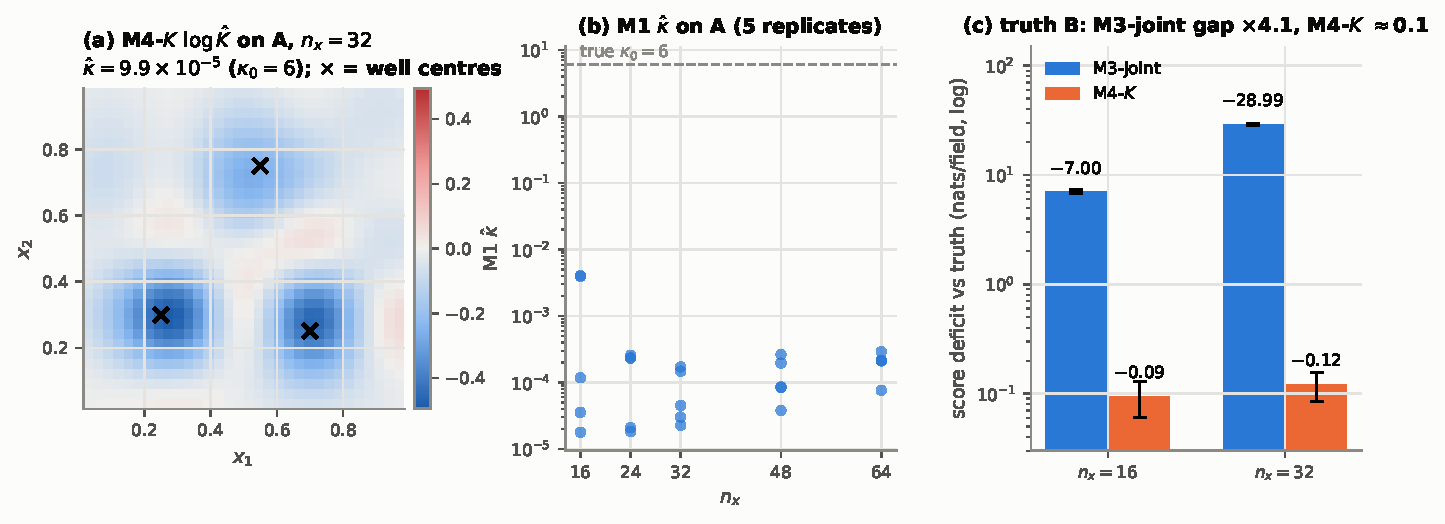
\includegraphics[width=\linewidth]{figures/fig5_3_misattribution.pdf}
    \caption{Misattribution by wrong-class models. (a) M4-$K$ fitted to truth A at $n_x=32$ places conductivity structure around the wells and collapses the range ($\widehat\kappa=9.9\times10^{-5}$). (b) M1 drives $\widehat\kappa$ toward zero on A at every grid. (c) On truth B, the held-out deficit of M3-joint grows from $7.00$ to $28.99$ nats per field as $N$ grows fourfold, while M4-$K$ remains near $-0.1$. Error bars are paired standard errors.}
    \label{fig:F5_3}
\end{figure}

\begin{table}[htbp]
\centering
\caption{Held-out log-likelihood relative to the truth (nats per field, 100 test fields; $0$ = truth) at $n_x=16$ and $32$. Superscript: CV-selected rank. Bold: best model. $\times$: gap growth, score at 32 divided by score at 16 ($N$ grows $4\times$).}
\label{tab:T5_3}
\fitbox{%
\begin{tabular}{@{}lrrrrrrrrrrrr@{}}
\toprule
 & \multicolumn{3}{c}{A} & \multicolumn{3}{c}{B$'$} & \multicolumn{3}{c}{B} & \multicolumn{3}{c}{C} \\
\cmidrule(lr){2-4} \cmidrule(lr){5-7} \cmidrule(lr){8-10} \cmidrule(lr){11-13}
Model & 16 & 32 & $\times$ & 16 & 32 & $\times$ & 16 & 32 & $\times$ & 16 & 32 & $\times$ \\
\midrule
M1 & -53.10 & -60.80 & 1.15 & -0.12 & -0.14 & 1.11 & -7.00 & -28.99 & 4.14 & -60.32 & -81.96 & 1.36 \\
M2 & -39.14 & -40.84 & 1.04 & -0.11 & -0.14 & 1.28 & -6.99 & -28.98 & 4.14 & -47.06 & -66.39 & 1.41 \\
M3-joint & \textbf{-1.76}$^{(3)}$ & \textbf{-5.78}$^{(3)}$ & 3.27 & -0.12$^{(0)}$ & -0.14$^{(0)}$ & 1.11 & -7.00$^{(0)}$ & -28.99$^{(0)}$ & 4.14 & -8.44$^{(3)}$ & -34.97$^{(3)}$ & 4.15 \\
M3-nested & -13.34$^{(3)}$ & -10.68$^{(3)}$ & 0.80 & -0.12$^{(0)}$ & -0.14$^{(0)}$ & 1.11 & -7.00$^{(0)}$ & -28.99$^{(0)}$ & 4.14 & -22.58$^{(3)}$ & -39.52$^{(3)}$ & 1.75 \\
M4-$\kappa$ & -46.56 & -60.80 & 1.31 & \textbf{0.01} & \textbf{0.00} & 0.09 & -5.90 & -26.54 & 4.50 & -54.84 & -78.50 & 1.43 \\
M4-$K$ & -31.11 & -47.42 & 1.52 & -0.11 & -0.25 & 2.30 & -0.09 & \textbf{-0.12} & 1.28 & -30.40 & -42.24 & 1.39 \\
M5 & -1.83$^{(3)}$ & -5.86$^{(3)}$ & 3.20 & -0.11$^{(0)}$ & -0.25$^{(0)}$ & 2.30 & \textbf{-0.09}$^{(0)}$ & -0.12$^{(0)}$ & 1.28 & \textbf{-1.83}$^{(3)}$ & \textbf{-6.37}$^{(3)}$ & 3.49 \\
\bottomrule
\multicolumn{13}{@{}p{0.97\linewidth}}{\footnotesize Paired standard errors (CSV) range from 0.03 to 5.6 nats; largest for the misspecified models on A and C. On B$'$, all models are within $\le 0.06$ nats standard error, so the apparent $0.01/0.00$ advantage of M4-$\kappa$ is not treated as a significant ranking and the growth ratio is not meaningful.} \\
\end{tabular}}
\end{table}

\begin{table}[htbp]
\centering
\caption{Operator recovery. corr $=\mathrm{corr}(\log\hat K,\log K_{\rm true})$ and peak $\hat K$ (true peak $e=2.718$) for M4-$K$ and M5 on B and C. Range: $\hat K$ for M4-$K$, M5; $\kappa(x)^2/\hat\kappa^2$ for M4-$\kappa$.}
\label{tab:T5_4}
\fitbox{%
\begin{tabular}{@{}llrrrrrrrrrr@{}}
\toprule
 & & \multicolumn{5}{c}{$n_x=16$} & \multicolumn{5}{c}{$n_x=32$} \\
\cmidrule(lr){3-7}\cmidrule(lr){8-12}
Truth & Model & $\hat\kappa$ & corr & peak $\hat K$ & range & $r_{\rm cv}$ & $\hat\kappa$ & corr & peak $\hat K$ & range & $r_{\rm cv}$ \\
\midrule
A & M1 & $7.17\times10^{-5}$ & --- & --- & --- & --- & $3.05\times10^{-5}$ & --- & --- & --- & --- \\
 & M3-joint & 6.18 & --- & --- & --- & 3 & 6.21 & --- & --- & --- & 3 \\
 & M4-$\kappa$ & 18.47 & --- & --- & 0.000337--0.668 & --- & $4.45\times10^{-5}$ & --- & --- & 0.999--1 & --- \\
 & M4-$K$ & $5.44\times10^{-5}$ & --- & --- & 0.31--1.01 & --- & $9.93\times10^{-5}$ & --- & --- & 0.61--1.06 & --- \\
 & M5 & 6.29 & --- & --- & 0.999--1.07 & 3 & 6.08 & --- & --- & 0.943--0.983 & 3 \\
\midrule
B$'$ & M1 & 5.54 & --- & --- & --- & --- & 5.44 & --- & --- & --- & --- \\
 & M3-joint & 5.54 & --- & --- & --- & 0 & 5.44 & --- & --- & --- & 0 \\
 & M4-$\kappa$ & 6.20 & --- & --- & 0.243--1.36 & --- & 3.24 & --- & --- & 0.478--7.12 & --- \\
 & M4-$K$ & 5.66 & --- & --- & 0.994--1.1 & --- & 5.51 & --- & --- & 1--1.06 & --- \\
 & M5 & 5.66 & --- & --- & 0.994--1.1 & 0 & 5.51 & --- & --- & 1--1.06 & 0 \\
\midrule
B & M1 & 6.02 & --- & --- & --- & --- & 6.05 & --- & --- & --- & --- \\
 & M3-joint & 6.02 & --- & --- & --- & 0 & 6.05 & --- & --- & --- & 0 \\
 & M4-$\kappa$ & 1.07 & --- & --- & 0.0121--126 & --- & 0.48 & --- & --- & 1.31--857 & --- \\
 & M4-$K$ & 5.93 & 0.997 & 2.46 & 0.923--2.46 & --- & 5.99 & 0.999 & 2.67 & 0.981--2.67 & --- \\
 & M5 & 5.93 & 0.997 & 2.46 & 0.923--2.46 & 0 & 5.99 & 0.999 & 2.67 & 0.981--2.67 & 0 \\
\midrule
C & M1 & $3.07\times10^{-5}$ & --- & --- & --- & --- & $1.77\times10^{-4}$ & --- & --- & --- & --- \\
 & M3-joint & 5.84 & --- & --- & --- & 3 & 6.18 & --- & --- & --- & 3 \\
 & M4-$\kappa$ & 31.88 & --- & --- & 0.000195--0.242 & --- & 5.63 & --- & --- & 2.04e-09--2.94 & --- \\
 & M4-$K$ & $3.66\times10^{-5}$ & 0.613 & 2.43 & 0.312--2.43 & --- & $1.11\times10^{-4}$ & 0.886 & 2.75 & 0.652--2.75 & --- \\
 & M5 & 5.77 & 0.997 & 2.52 & 0.956--2.52 & 3 & 6.06 & 0.999 & 2.61 & 0.953--2.61 & 3 \\
\bottomrule
\multicolumn{12}{@{}p{0.97\linewidth}}{\footnotesize corr is left blank on A and B$'$: their true conductivity is $K\equiv1$, so $\log K_{\rm true}$ is constant and the correlation is undefined. M4-$\kappa$ on B: the extreme range $\kappa(x)^2/\hat\kappa^2$ is a converged fit, not an optimiser failure (433 and 597 iterations; final gradient $1.5\times10^{-5}$ and $4.3\times10^{-5}$ per field; restarting L-BFGS from the stored point lowers the objective by $<10^{-10}$ per field; \texttt{data/check\_m4kappa\_B.json}). It is the zeroth-order model's best imitation of a principal-part change (single start).} \\
\end{tabular}}
\end{table}

\begin{table}[htbp]
\centering
\caption{Spike recovery on A and C (true $c=90/60/40$). $\hat c_k=\hat s_k-1$; per-well cosines and principal-angle cosines to the true 3-d well span.}
\label{tab:T5_4b}
\fitbox{%
\begin{tabular}{@{}lllrlll@{}}
\toprule
Truth & Model & $n_x$ & $r_{\rm MP}$ & $\hat c_{1..3}$ & $\cos_{1..3}$ & span cosines \\
\midrule
A & M3-joint & 16 & 3 & 99.2/62.5/41.6 & 0.945/0.945/0.979 & 0.994/0.990/0.985 \\
 &  & 32 & 4 & 101.8/77.3/47.6 & 0.955/0.946/0.938 & 0.973/0.964/0.941 \\
 & M3-nested & 16 & 3 & 46.4/28.8/19.1 & 0.924/0.920/0.952 & 0.977/0.970/0.953 \\
 &  & 32 & 3 & 63.1/47.2/29.9 & 0.918/0.905/0.895 & 0.946/0.931/0.896 \\
 & M5 & 16 & --- & 98.8/61.4/41.5 & 0.947/0.947/0.979 & 0.994/0.989/0.985 \\
 &  & 32 & --- & 102.8/75.9/47.7 & 0.958/0.948/0.938 & 0.973/0.963/0.941 \\
\midrule
C & M3-joint & 16 & 4 & 116.4/68.8/41.9 & 0.987/0.984/0.977 & 0.992/0.989/0.978 \\
 &  & 32 & 4 & 112.6/65.6/46.0 & 0.875/0.859/0.934 & 0.974/0.955/0.936 \\
 & M3-nested & 16 & 3 & 53.1/31.2/18.8 & 0.964/0.958/0.951 & 0.974/0.964/0.951 \\
 &  & 32 & 3 & 69.1/41.7/28.6 & 0.853/0.834/0.894 & 0.941/0.922/0.894 \\
 & M5 & 16 & --- & 109.7/66.0/44.1 & 0.987/0.984/0.984 & 0.994/0.990/0.985 \\
 &  & 32 & --- & 104.5/62.0/48.5 & 0.875/0.858/0.945 & 0.975/0.954/0.946 \\
\bottomrule
\multicolumn{7}{@{}p{0.97\linewidth}}{\footnotesize M3 cosines are from the rank-3 fit (the CV choice is 3 in every case shown). $r_{\rm MP}$ is counted after whitening by each model's own base: the fitted M1 for M3-nested, as in Table~\ref{tab:T5_2}, and the jointly fitted base ($\hat\kappa\approx6$) for M3-joint, under which one further eigenvalue crosses the unmodified edge in three cases. These counts come from the single main-seed ensemble, not the five replicates of Table~\ref{tab:T5_2}. M5 has no $r_{\rm MP}$ (rank by CV only).} \\
\end{tabular}}
\end{table}

\subsection{The combined model separates source and operator variability}
\label{sec:results_m5}

M5 is intended to prevent the compensating failures above by learning the principal operator and the finite-rank correction together. Figure~\ref{fig:F5_4} shows that the two components are used selectively rather than both being activated indiscriminately. In the diagnostic control at $n_x=32$, deflation removed about one upper-edge direction on B, where these are sampling fluctuations, and exactly three on C, where they are the source directions (Table~\ref{tab:T5_2}).

On A, CV selects $r=3$, the fitted conductivity remains nearly flat, and the range returns to $\widehat\kappa=6.08$ at $n_x=32$; on the same data M1 alone gives $3.0\times10^{-5}$, so allowing the source component moves the inferred range by about five orders of magnitude back to $\kappa_0=6$. The held-out score and the recovered source subspace are essentially those of M3-joint (Tables~\ref{tab:T5_3} and~\ref{tab:T5_4b}), so the extra operator component does not create spurious conductivity structure when the source correction already explains the variation. On B, CV selects $r=0$, the finite-rank component switches off, and the fit coincides with M4-$K$, as expected when no source correction is required. On C both components are needed: M5 selects $r=3$, recovers the conductivity shape and the reference range, and retains a three-dimensional source subspace, with a held-out deficit several times smaller than those of M3-joint and M4-$K$. The gain is not simply additional flexibility: the decomposition simultaneously restores the reference range, the conductivity shape, and the finite-dimensional source subspace that each single-component model confounds.

M5 is not intended to replace the lower-order model. On B$'$, CV selects $r=0$ and the conductivity field stays close to flat, but M5 contains no spatially varying leakage coefficient and M4-$\kappa$ remains the matched model; M5 is a source-plus-principal architecture rather than a universal covariance approximator. The exact block-coordinate implementation leaves the conclusions unchanged relative to the earlier legacy alternation (Table~\ref{tab:T5_5}): on C at $n_x=32$ the held-out score changes only from $-6.377$ to $-6.373$ nats per field and the conductivity correlation remains $0.9994$, while $\widehat\kappa$ moves from $5.95$ to $6.06$, so the correction affects the internal consistency of the decomposition more than the model comparison.

\begin{figure}[htbp]
    \centering
    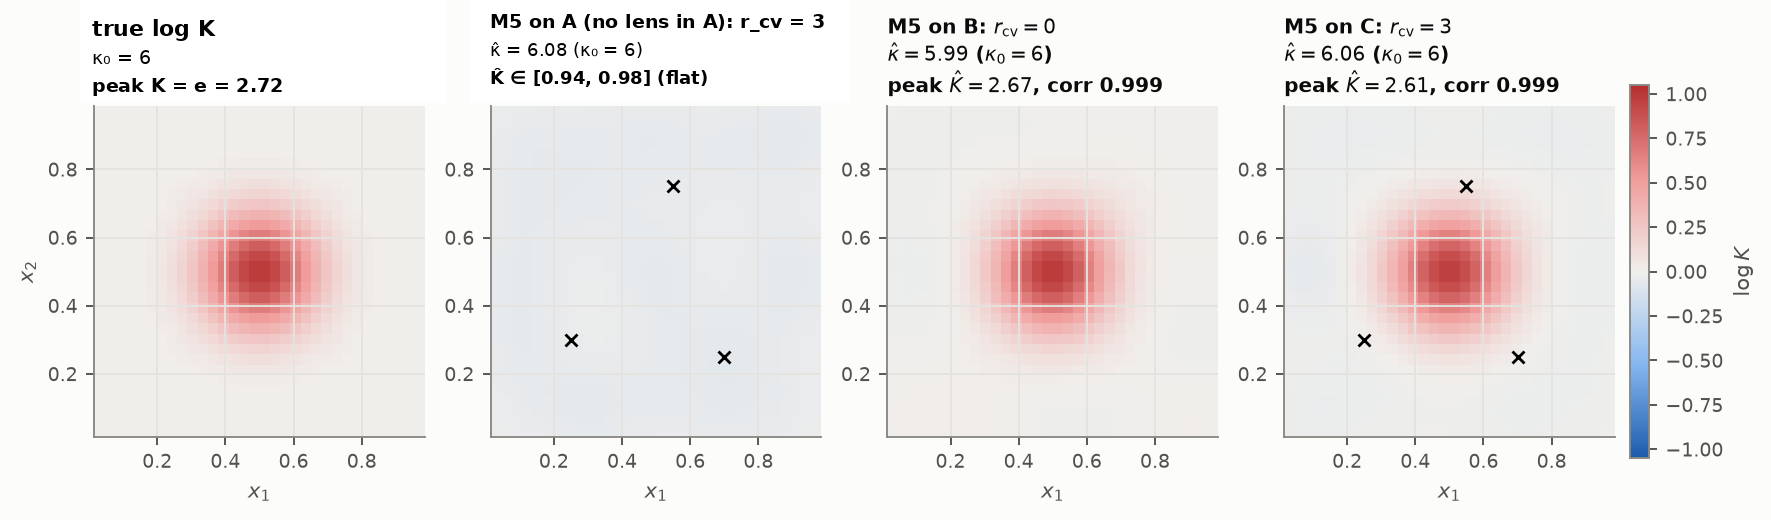
\includegraphics[width=\linewidth]{figures/fig5_4_m5_selectivity.png}
    \caption{M5 selectivity at $n_x=32$: learned $\log\widehat K$ and CV rank ($\kappa_0=6$; true peak $K=e$). The first panel shows the true $\log K$ used in truths B and C; truth A has no conductivity lens. A: $r=3$, $\widehat\kappa=6.08$, nearly flat $\widehat K$. B: $r=0$, $\widehat\kappa=5.99$, peak $\widehat K=2.67$. C: $r=3$, $\widehat\kappa=6.06$, peak $\widehat K=2.61$.}
    \label{fig:F5_4}
\end{figure}

\FloatBarrier
\subsection{Robustness}
\label{sec:robustness}

The conclusions survive each robustness check; the tables are collected in Appendix~\ref{app:robustness}. Across the main seed and three fresh seeds at $n_x=32$, M5 selects ranks $3$, $0$ and $3$ on A, B and C (Table~\ref{tab:r-seeds}). Moving the lens off the RBF grid increases the M5 deficits on B and C and lowers the lens correlation to about $0.974$, but leaves the rank allocation unchanged. Sweeping $\lambda_\theta$ from $10^{-3}$ to $10$ leaves the B and C correlations, ranks, and scores unchanged at the reported precision (Table~\ref{tab:r-lambda}). Cross-fitting the whitening and deflation on independent 100-field halves preserves the plateau on B and C and the decay on A (Table~\ref{tab:r-crossfit}), so the separation does not depend on same-sample fitting. Increasing the B$'$ ensemble from $200$ to $800$ fields raises the M4-$\kappa$ leakage correlation while all score differences stay below $0.15$ nats per field (Table~\ref{tab:r-bp}): the weak lower-order case becomes more recoverable with replication. With ten sensors at $5\%$ noise, M5 on C keeps a posterior-mean RMSE close to that of the truth and a conditional deficit several times smaller than M3-joint or M4-$K$ (Table~\ref{tab:r-sensors}), so the mechanism allocation remains useful under sparse conditioning.

The principal-part signature also persists for coefficients other than the smooth lens (Table~\ref{tab:r-disc}). For the discontinuous disc lens, which Lemma~\ref{lem:mult_compact} does not cover, $D_N/N$ stays non-vanishing and $\mathrm{KL}_N$ grows linearly. The constant rescaling $K\equiv1.5$ gives a second, independent check of the lemma's plateau constant: here $m=K^{-2}-1$ is constant, so the lemma predicts $D_N/N\to(1/2.25-1)^2=0.3086$, and the computed values rise from $0.2919$ to $0.3070$ toward it. Its KL slope agrees likewise: $\mathrm{KL}_N/N=0.1268$ at $n_x=64$ against the predicted $\tfrac12[m-\log(1+m)]=0.1277$. The lemma's constants are thus checked on two principal-part departures of different form.

\FloatBarrier
\section{Discussion and conclusion}
\label{sec:discussion}

The central result is that replicated fields can decide whether a discrepancy from a Gaussian reference should be represented as a correction of that reference or as a change in its covariance-generating operator. Source and lower-order departures produced refinement behavior consistent with the reference measure class, a principal-coefficient change produced persistent relative covariance energy and an extensive KL cost, and $\widehat h_N$ turned this distinction into a sample quantity that, for the lens, tracked the oracle sequence and the predicted $h_\infty$. Wrong-class models did not merely lose score; they reassigned variability to plausible but incorrect components, and M5, given both components, allocated each form of variability to the right one.

The resulting modeling rule is: \emph{learn the operator where the population demands a change of Gaussian measure class; correct relative to that operator where the remaining discrepancy stays within class}. When a discrepancy persists across an increasing fraction of resolved modes, adding correction terms to a fixed reference does not address it; the reference itself must change.

\paragraph{Implications for learned priors and function-space generative models.}
Discretization-independent generative constructions already make absolute-continuity and Cameron--Martin assumptions explicit \citep{Lim2025,Pidstrigach2023}. If the principal part of the Gaussian reference is wrong, no finite-dimensional correction repairs the measure-class mismatch, even though a fixed mesh can make the corrected covariance look adequate. A refinement diagnostic of the type used here can serve as a pre-training check on the reference.

\paragraph{Implications for reference-based complexity priors.}
For a principal-part mismatch, $\mathrm{KL}_N=O(N)$, so the PC distance $d_N=\sqrt{2\,\mathrm{KL}_N}$ grows as $O(\sqrt N)$ and the same physical departure looks more complex as the mesh is refined \citep{Simpson2017,Fuglstad2019}. A discretization-stable complexity then needs either a different distance, as for singular operator changes \citep{LlamazaresElias2026}, or a new base operator relative to which the remaining departure is within class.

\paragraph{Implications for spatial covariance fitting.}
With unmodeled wells, the stationary fit gives $\widehat\kappa\approx3\times10^{-5}$ against a generating value of $6$, while M5 returns $\widehat\kappa=6.08$. The base of the Mat\'ern PC prior for the range is infinite range, $\kappa=0$ \citep{Fuglstad2019}, so shrinkage toward it would reinforce the confounded direction. A near-zero fitted range when sources may be unmodeled is a mechanism-attribution warning, not automatically evidence of long-range dependence.

\paragraph{Limitations.}
Several robustness checks in Section~\ref{sec:robustness} reduce implementation-specific concerns: although $\lambda_\theta$ was fixed by hand, sweeping it from $10^{-3}$ to $10$ leaves the B and C M5 ranks and scores unchanged at the reported precision; across four seeds the $n_x=32$ M5 ranks remain $3/0/3$ for A/B/C; moving the lens off the RBF grid lowers the fitted lens correlation to about $0.974$ but preserves the B/C rank allocation; a discontinuous disc lens retains non-vanishing $D_N/N$ and a growing KL cost; and the constant rescaling $K\equiv1.5$ likewise retains extensive principal-part scaling. The remaining limitations are structural. The source-deflation rule was evaluated with a stiff conductivity lens, $K\ge1$, so although the diagonal refinement statistic $h_N$ is sign insensitive, the upper-edge source-removal step is not yet a general soft-lens classifier. The study is two-dimensional and employs a square domain whose corners fall outside the smooth-boundary assumptions of the strongest variable-coefficient equivalence theorem. M5 does not include a spatially varying lower-order coefficient, and M4 fits use a single initialization. No real aquifer data are analyzed, and the sample-based diagonal refinement statistic $\widehat h_N$ and M5 architecture were developed after the oracle refinement results rather than specified in advance.

\paragraph{Next steps.}
A soft-lens experiment would separate the sign-insensitive diagnostic from the sign-specific deflation rule, and low-replicate regimes would show how much replication the classification needs. Lemma~\ref{lem:mult_compact} should be extended to discontinuous coefficients, as the disc lens suggests, to tensor-valued $K$, and to $d=3$. Samplers for principal-part hyperparameters, which index mutually singular families, deserve study under refinement. Finally, the approach should be tested on replicated observations from a pumped heterogeneous aquifer, and on population priors over constitutive behavior transferred between experiments in mechanics.

The opening question can therefore be answered empirically: whether to correct a Gaussian reference or change its operator is a question that replicated data can answer, and getting that decision wrong can produce a confident, physically plausible, but structurally incorrect model.

\FloatBarrier
\appendix

\section{Proof of Proposition~\ref{prop:refinement}}
\label{app:proof_refinement}

\begin{proof}
If $T\in\mathcal S_2$ and $P_N\to I$ strongly, then finite-rank compression converges in Hilbert--Schmidt norm,
\begin{equation}
    \|P_NTP_N-T\|_{\mathrm{HS}}\longrightarrow0.
\end{equation}
Therefore
\begin{equation}
    D_N
    =
    \|P_NTP_N\|_{\mathrm{HS}}^2
    \longrightarrow
    \|T\|_{\mathrm{HS}}^2<\infty.
\end{equation}
Since the numerator converges to a finite limit while $N\to\infty$,
\begin{equation}
    \frac{D_N}{N}\longrightarrow0. \qedhere
\end{equation}
\end{proof}

\section{Proof of Lemma~\ref{lem:mult_compact}}
\label{app:proof_lemma}

\begin{proof}
Write $\mathcal K$ for the compact operators on $L^2(\mathcal D)$.

\emph{Step 1 (regularity).} For a smooth or convex polygonal domain and $K\in C^1(\overline{\mathcal D})$, $K\ge k_0>0$, both $A_0^{-1}$ and $A_1^{-1}$ map $L^2(\mathcal D)$ boundedly into $H^2(\mathcal D)\cap H^1_0(\mathcal D)$. Hence $A_0A_1^{-1}$ and $A_1A_0^{-1}$ extend to bounded operators on $L^2(\mathcal D)$, and each is the inverse of the other.

\emph{Step 2 ($A_1A_0^{-1}=M_K+\mathcal K$).} Let $B=A_1-A_0=-\nabla\!\cdot((K-1)\nabla)=-(K-1)\Delta-\nabla K\cdot\nabla$. Since $-\Delta A_0^{-1}=I-\kappa^2A_0^{-1}$,
\begin{equation}
    BA_0^{-1}=M_{K-1}-\kappa^2M_{K-1}A_0^{-1}-(\nabla K\cdot\nabla)A_0^{-1}.
\end{equation}
The operator $A_0^{-1}$ is compact on $L^2$, and $\nabla A_0^{-1}$ maps $L^2$ boundedly into $H^1$, which embeds compactly into $L^2$ (Rellich). Multiplication by the bounded functions $K-1$ and $\nabla K$ preserves compactness. Hence $BA_0^{-1}=M_{K-1}+C_1$ with $C_1\in\mathcal K$, and $A_1A_0^{-1}=I+BA_0^{-1}=M_K+C_1$.

\emph{Step 3 ($A_0A_1^{-1}=M_{1/K}+\mathcal K$).} Let $G=A_0A_1^{-1}$. From $(M_K+C_1)G=I$,
\begin{equation}
    G=M_{1/K}-M_{1/K}C_1G=M_{1/K}+C_2,
    \qquad
    C_2\in\mathcal K.
\end{equation}

\emph{Step 4 (the decomposition).} Since $\Sigma_0^{-1/2}=c^{-1/2}A_0$ and $\Sigma_1=c\,A_1^{-2}$, and $A_0,A_1$ are self-adjoint,
\begin{equation}
    T+I=A_0A_1^{-1}A_1^{-1}A_0=GG^*=(M_{1/K}+C_2)(M_{1/K}+C_2^*)=M_{1/K^2}+C_3,
    \qquad
    C_3\in\mathcal K,
\end{equation}
which is \eqref{eq:mult_compact} with $R=C_3$. Since $G$ is invertible, $T+I\ge\gamma I$ for some $\gamma>0$.

\emph{(i).} By Weyl's theorem, compact perturbations do not change the essential spectrum, so $\sigma_{\rm ess}(T)=\sigma_{\rm ess}(M_m)$, the essential range of $m$, which equals $m(\overline{\mathcal D})$ for continuous $m$. A compact operator has essential spectrum $\{0\}$, so $T$ is compact only if $m\equiv0$, i.e.\ $K\equiv1$.

\emph{(ii).} In the orthonormal basis of normalized cell indicators, $P_NM_mP_N$ is diagonal with entries the cell averages $\bar m_i$, so $\frac1N\|P_NM_mP_N\|_{\rm HS}^2=\frac1N\sum_i\bar m_i^2\to|\mathcal D|^{-1}\int m^2$ by uniform continuity of $m$. For the remainder, $P_NRP_N$ has rank at most $N$ and singular values $s_j(P_NRP_N)\le s_j(R)$, so
\begin{equation}
    \frac1N\|P_NRP_N\|_{\rm HS}^2\le\frac1N\sum_{j=1}^{N}s_j(R)^2\longrightarrow0,
\end{equation}
because $s_j(R)\to0$ and Ces\`aro means of a null sequence vanish. The cross term vanishes by Cauchy--Schwarz, giving the first limit in \eqref{eq:lemma_energy}. The diagonal entries of $T_N$ are $\bar m_i+(P_NRP_N)_{ii}$ with $\frac1N\sum_i(P_NRP_N)_{ii}^2\le\frac1N\|P_NRP_N\|_{\rm HS}^2\to0$, giving the second limit. Because $P_NM_mP_N$ has no off-diagonal entries in this basis, the difference of the two quantities tends to zero.

\emph{(iii).} By the Hoffman--Wielandt inequality, with eigenvalues and cell averages both sorted,
\begin{equation}
    \frac1N\sum_{j=1}^{N}\big|t_{j,N}-\bar m_{(j)}\big|^2\le\frac1N\|P_NRP_N\|_{\rm HS}^2\longrightarrow0,
\end{equation}
so the empirical eigenvalue distribution of $T_N$ has the same weak limit as that of the $\bar m_i$, namely the law of $m(X)$. The persistent-mode statement follows at every $\delta$ with $|\{|m|=\delta\}|=0$. Finally, all $t_{j,N}$ and $\bar m_i$ lie in a compact interval $[\gamma'-1,\|T\|]$ with $\gamma'=\min(\gamma,\min K^{-2})>0$, on which $f(t)=t-\log(1+t)$ is Lipschitz; hence $\frac1N\sum_jf(t_{j,N})-\frac1N\sum_if(\bar m_i)\to0$, and the second sum tends to $|\mathcal D|^{-1}\int f(m)$. This gives \eqref{eq:lemma_kl}.
\end{proof}

\section{Optimization settings}
\label{app:optimization}

\begin{table}[H]
\centering
\caption{Optimiser settings (L-BFGS-B, SciPy; gradients by JAX autodiff).}
\label{tab:tolerances}
\fitbox{%
\begin{tabular}{@{}llll@{}}
\toprule
Model & Inner solve & Outer loop & Other \\
\midrule
M1, M2 & maxiter 1000, maxfun 3000, gtol $10^{-8}$, ftol $10^{-13}$ & --- & --- \\
M4-$\kappa$, M4-$K$ & maxiter 2000, maxfun 6000, gtol $10^{-8}$, ftol $10^{-13}$ & --- & dense Cholesky \\
M3-joint & maxiter 500, gtol $10^{-10}$, ftol $10^{-15}$ & $\Delta\ell<10^{-9}$ per field, $\le1000$ & 2 starts \\
M5 & maxiter 500, gtol $10^{-8}$, ftol $10^{-14}$ & $\Delta\ell<10^{-7}n$ per cycle, $\le60$ & monotone check, slack $10^{-8}n$ \\
\midrule
\multicolumn{4}{@{}l}{$\kappa$ floored at $10^{-3}$ at initialisation only; no bounds during optimisation.} \\
\bottomrule
\end{tabular}}
\end{table}

\section{Robustness tables}
\label{app:robustness}

\begin{table}[H]
\centering
\caption{Oracle refinement for the disc lens and constant $K\equiv1.5$ (smooth lens B in Table~\ref{tab:T5_1}). For constant $K$, Lemma~\ref{lem:mult_compact} predicts $D_N/N\to(K^{-2}-1)^2=0.3086$.}
\label{tab:r-disc}
\begin{tabular}{@{}llrrr@{}}
\toprule
Truth & $n_x$ & $D_N/N$ & KL$_N$ & $W_2$ \\
\midrule
B\_disk & 16 & 0.0325 & 5.21 & 0.0030 \\
 & 24 & 0.0403 & 15.87 & --- \\
 & 32 & 0.0374 & 26.73 & 0.0033 \\
 & 48 & 0.0362 & 59.80 & --- \\
 & 64 & 0.0351 & 104.30 & 0.0032 \\
K\_const & 16 & 0.2919 & 30.39 & 0.0093 \\
 & 24 & 0.2999 & 70.81 & --- \\
 & 32 & 0.3032 & 127.70 & 0.0090 \\
 & 48 & 0.3059 & 290.71 & --- \\
 & 64 & 0.3070 & 519.22 & 0.0089 \\
\bottomrule
\end{tabular}
\end{table}

\begin{table}[H]
\centering
\caption{Ten sensors, 5\,\% noise, $n_x=32$: conditional log predictive density $\log p(u_{\rm test}\mid y)$ of the full field given the sensor readings, relative to the truth (nats per field), and RMSE of the posterior mean field.}
\label{tab:r-sensors}
\fitbox{%
\begin{tabular}{@{}lrrrrrrrr@{}}
\toprule
Model & A lpd & A RMSE & B$'$ lpd & B$'$ RMSE & B lpd & B RMSE & C lpd & C RMSE \\
\midrule
truth & 0.00 & 0.0347 & 0.00 & 0.0266 & 0.00 & 0.0239 & 0.00 & 0.0314 \\
M1 & -58.89 & 0.0564 & -0.09 & 0.0266 & -28.89 & 0.0240 & -80.28 & 0.0494 \\
M2 & -37.07 & 0.0562 & -0.11 & 0.0267 & -28.89 & 0.0240 & -62.87 & 0.0496 \\
M3-joint & -5.77 & 0.0348 & -0.09 & 0.0266 & -28.89 & 0.0240 & -34.89 & 0.0318 \\
M3-nested & -9.87 & 0.0358 & -0.09 & 0.0266 & -28.89 & 0.0240 & -38.65 & 0.0327 \\
M4-$\kappa$ & -58.89 & 0.0564 & -0.02 & 0.0266 & -26.07 & 0.0247 & -76.15 & 0.0497 \\
M4-$K$ & -45.38 & 0.0563 & -0.20 & 0.0266 & -0.12 & 0.0239 & -40.38 & 0.0501 \\
M5 & -5.85 & 0.0348 & -0.20 & 0.0266 & -0.12 & 0.0239 & -6.29 & 0.0316 \\
\bottomrule
\end{tabular}}
\end{table}

\begin{table}[H]
\centering
\caption{Truth B$'$ with more training fields (nested: the main 200 plus new fields; main test set). Scores in nats per field vs truth; M4-$\kappa$ corr with the true $\log(\kappa(x)^2/\kappa_0^2)$.}
\label{tab:r-bp}
\begin{tabular}{@{}rrrrrrrrr@{}}
\toprule
$n_x$ & $n_{\rm train}$ & M1 & M1 $\hat\kappa$ & M3-joint & $r_{\rm cv}$ & $r_{\rm MP}$ & M4-$\kappa$ & corr \\
\midrule
16 & 200 & -0.125 & 5.54 & -0.125 & 0 & 0 & 0.007 & 0.738 \\
16 & 400 & -0.133 & 5.64 & -0.133 & 0 & 0 & -0.024 & 0.856 \\
16 & 800 & -0.138 & 5.56 & -0.138 & 0 & 0 & -0.042 & 0.929 \\
32 & 200 & -0.138 & 5.44 & -0.138 & 0 & 0 & 0.001 & 0.800 \\
32 & 400 & -0.144 & 5.49 & -0.144 & 0 & 0 & -0.038 & 0.861 \\
32 & 800 & -0.148 & 5.52 & -0.148 & 0 & 0 & -0.025 & 0.874 \\
\bottomrule
\end{tabular}
\end{table}

\begin{table}[H]
\centering
\caption{Robustness: held-out score vs truth (nats per field) over the main seed and three fresh seeds (mean $\pm$ s.d.), and the off-grid lens (centre $(0.42,0.57)$). M5 exact everywhere.}
\label{tab:r-seeds}
\fitbox{%
\begin{tabular}{@{}lllrrrrrrl@{}}
\toprule
Truth & $n_x$ & seeds & M1 & M2 & M3-joint & M4-$\kappa$ & M4-$K$ & M5 & M5 $r_{\rm cv}$ \\
\midrule
A & 16 & 4 & -52.45$\pm$1.81 & -39.32$\pm$1.14 & -1.74$\pm$0.23 & -45.61$\pm$1.52 & -30.40$\pm$0.99 & -1.81$\pm$0.24 & 3 \\
A & 32 & 4 & -60.64$\pm$2.00 & -40.27$\pm$0.89 & -6.97$\pm$0.86 & -58.21$\pm$2.46 & -47.17$\pm$1.30 & -7.04$\pm$0.86 & 3 \\
B$'$ & 16 & 4 & -0.07$\pm$0.03 & -0.08$\pm$0.02 & -0.07$\pm$0.03 & -0.05$\pm$0.04 & -0.12$\pm$0.02 & -0.12$\pm$0.02 & 0 \\
B$'$ & 32 & 4 & -0.12$\pm$0.03 & -0.13$\pm$0.01 & -0.12$\pm$0.03 & -0.04$\pm$0.05 & -0.16$\pm$0.06 & -0.16$\pm$0.06 & 0 \\
B & 16 & 4 & -6.82$\pm$0.20 & -6.82$\pm$0.21 & -6.82$\pm$0.20 & -5.47$\pm$0.28 & -0.09$\pm$0.02 & -0.09$\pm$0.02 & 0 \\
B & 32 & 4 & -28.47$\pm$0.68 & -28.47$\pm$0.69 & -28.47$\pm$0.68 & -25.98$\pm$0.65 & -0.10$\pm$0.02 & -0.10$\pm$0.02 & 0 \\
C & 16 & 4 & -57.54$\pm$2.04 & -45.32$\pm$1.30 & -8.36$\pm$0.16 & -51.85$\pm$2.03 & -29.36$\pm$0.96 & -1.98$\pm$0.30 & 3 \\
C & 32 & 4 & -88.01$\pm$4.32 & -68.57$\pm$1.79 & -35.47$\pm$0.44 & -84.86$\pm$5.08 & -46.04$\pm$2.66 & -7.14$\pm$0.50 & 3 \\
B off-grid & 16 & 1 & -6.99 & -6.99 & -6.99 & -5.69 & -0.37 & -0.37 & 0 \\
C off-grid & 16 & 1 & -60.06 & -46.83 & -8.67 & -54.55 & -31.29 & -2.15 & 3 \\
B off-grid & 32 & 1 & -28.63 & -28.62 & -28.63 & -26.19 & -1.73 & -1.73 & 0 \\
C off-grid & 32 & 1 & -81.62 & -65.75 & -34.36 & -80.65 & -44.67 & -7.91 & 3 \\
\bottomrule
\multicolumn{10}{@{}p{0.97\linewidth}}{\footnotesize M3-nested was not refitted on the robustness seeds (\texttt{run\_robust\_fits.py} skips it); it is omitted here.} \\
\end{tabular}}
\end{table}

\begin{table}[H]
\centering
\caption{M5: exact block coordinate ascent vs the legacy alternation (legacy shown for comparison only). Cycles and final gradient norm $\|\nabla_{(\log\kappa,\theta)}\|$ of the total objective ($n_{\rm train}=200$) for the exact fit; the legacy run did not record them.}
\label{tab:T5_5}
\fitbox{%
\begin{tabular}{@{}llrrcrrrrrr@{}}
\toprule
Truth & $n_x$ & score (leg.) & score (exact) & $r_{\rm cv}$ & $\hat\kappa$ (leg.) & $\hat\kappa$ (exact) & corr (leg.) & corr (exact) & cycles & $\|\nabla\|$ \\
\midrule
A & 16 & -1.83 & -1.83 & 3/3 & 5.87 & 6.29 & --- & --- & 15 & 0.301 \\
B$'$ & 16 & -0.11 & -0.11 & 0/0 & 5.66 & 5.66 & --- & --- & 2 & 0.002 \\
B & 16 & -0.09 & -0.09 & 0/0 & 5.93 & 5.93 & 0.9970 & 0.9970 & 2 & 0.001 \\
C & 16 & -1.87 & -1.83 & 3/3 & 5.32 & 5.77 & 0.9965 & 0.9974 & 14 & 0.259 \\
A & 32 & -5.86 & -5.86 & 3/3 & 6.00 & 6.08 & --- & --- & 8 & 0.301 \\
B$'$ & 32 & -0.25 & -0.25 & 0/0 & 5.51 & 5.51 & --- & --- & 2 & 0.015 \\
B & 32 & -0.12 & -0.12 & 0/0 & 5.99 & 5.99 & 0.9990 & 0.9990 & 2 & 0.010 \\
C & 32 & -6.38 & -6.37 & 3/3 & 5.95 & 6.06 & 0.9994 & 0.9994 & 13 & 0.304 \\
\bottomrule
\multicolumn{11}{@{}p{0.97\linewidth}}{\footnotesize corr is omitted on A and B$'$, whose true conductivity is $K\equiv1$, so the correlation is undefined (as in Table~\ref{tab:T5_4}).} \\
\end{tabular}}
\end{table}

\begin{table}[H]
\centering
\caption{$\lambda_\theta$ sweep (penalty $\lambda_\theta\|\theta\|^2$ on the total negative log-likelihood). True peak $K=e=2.718$.}
\label{tab:r-lambda}
\fitbox{%
\begin{tabular}{@{}lllrrrrrrr@{}}
\toprule
Truth & $n_x$ & $\lambda_\theta$ & M4-$K$ corr & M4-$K$ $\max\hat K$ & M4-$K$ score & M5 corr & M5 $\max\hat K$ & M5 $r_{\rm cv}$ & M5 score \\
\midrule
B & 16 & 0.001 & 0.9970 & 2.46 & -0.09 & 0.9970 & 2.46 & 0 & -0.09 \\
B & 16 & 0.01 & 0.9970 & 2.46 & -0.09 & 0.9970 & 2.46 & 0 & -0.09 \\
B & 16 & 0.1 & 0.9970 & 2.46 & -0.09 & 0.9970 & 2.46 & 0 & -0.09 \\
B & 16 & 1 & 0.9970 & 2.45 & -0.09 & 0.9970 & 2.45 & 0 & -0.09 \\
B & 16 & 10 & 0.9973 & 2.40 & -0.08 & 0.9973 & 2.40 & 0 & -0.08 \\
B & 32 & 0.001 & 0.9990 & 2.67 & -0.12 & 0.9990 & 2.67 & 0 & -0.12 \\
B & 32 & 0.01 & 0.9990 & 2.67 & -0.12 & 0.9990 & 2.67 & 0 & -0.12 \\
B & 32 & 0.1 & 0.9990 & 2.67 & -0.12 & 0.9990 & 2.67 & 0 & -0.12 \\
B & 32 & 1 & 0.9990 & 2.67 & -0.12 & 0.9990 & 2.67 & 0 & -0.12 \\
B & 32 & 10 & 0.9990 & 2.65 & -0.12 & 0.9990 & 2.65 & 0 & -0.12 \\
C & 16 & 0.001 & 0.6131 & 2.43 & -30.40 & 0.9974 & 2.52 & 3 & -1.83 \\
C & 16 & 0.01 & 0.6131 & 2.43 & -30.40 & 0.9974 & 2.52 & 3 & -1.83 \\
C & 16 & 0.1 & 0.6131 & 2.43 & -30.40 & 0.9974 & 2.52 & 3 & -1.83 \\
C & 16 & 1 & 0.6134 & 2.44 & -30.39 & 0.9975 & 2.51 & 3 & -1.83 \\
C & 16 & 10 & 0.6159 & 2.50 & -30.38 & 0.9977 & 2.44 & 3 & -1.83 \\
C & 32 & 0.001 & 0.8864 & 2.75 & -42.24 & 0.9994 & 2.61 & 3 & -6.37 \\
C & 32 & 0.01 & 0.8864 & 2.75 & -42.24 & 0.9994 & 2.61 & 3 & -6.37 \\
C & 32 & 0.1 & 0.8864 & 2.75 & -42.24 & 0.9994 & 2.61 & 3 & -6.37 \\
C & 32 & 1 & 0.8864 & 2.75 & -42.23 & 0.9994 & 2.61 & 3 & -6.37 \\
C & 32 & 10 & 0.8868 & 2.74 & -42.22 & 0.9994 & 2.60 & 3 & -6.37 \\
\bottomrule
\end{tabular}}
\end{table}

\begin{table}[H]
\centering
\caption{Cross-fitted diagnostic: M1 whitening and deflation directions fitted on 100 fields, $\hat h_N$ computed on the other 100, swapped and averaged (5 replicates; same fields as Table~\ref{tab:T5_2}).}
\label{tab:r-crossfit}
\fitbox{%
\begin{tabular}{@{}llrrrr@{}}
\toprule
Truth & $n_x$ & $\hat h_N$ raw & $\hat h_N$ deflated & $r_{\rm MP}$ & in-sample deflated \\
\midrule
ref & 16 & 0.0008 $\pm$ 0.0010 & 0.0008 $\pm$ 0.0010 & 0.0 & 0.0002 \\
 & 24 & -0.0004 $\pm$ 0.0003 & -0.0004 $\pm$ 0.0003 & 0.2 & -0.0003 \\
 & 32 & 0.0003 $\pm$ 0.0005 & 0.0003 $\pm$ 0.0005 & 0.2 & 0.0001 \\
 & 48 & 0.0001 $\pm$ 0.0004 & 0.0001 $\pm$ 0.0004 & 0.4 & 0.0002 \\
 & 64 & $-4.26\times10^{-5}$ $\pm$ 0.0002 & $-4.04\times10^{-5}$ $\pm$ 0.0002 & 0.2 & $-2.93\times10^{-5}$ \\
\midrule
A & 16 & 3.2633 $\pm$ 0.2080 & 0.1236 $\pm$ 0.0089 & 3.0 & 0.1440 \\
 & 24 & 0.9234 $\pm$ 0.1263 & 0.0320 $\pm$ 0.0042 & 3.0 & 0.0445 \\
 & 32 & 0.3286 $\pm$ 0.0312 & 0.0102 $\pm$ 0.0008 & 3.0 & 0.0173 \\
 & 48 & 0.0787 $\pm$ 0.0079 & 0.0029 $\pm$ 0.0007 & 3.0 & 0.0050 \\
 & 64 & 0.0250 $\pm$ 0.0025 & 0.0018 $\pm$ 0.0003 & 3.0 & 0.0023 \\
\midrule
B$'$ & 16 & 0.0008 $\pm$ 0.0013 & 0.0008 $\pm$ 0.0013 & 0.0 & 0.0012 \\
 & 24 & $-7.24\times10^{-5}$ $\pm$ 0.0005 & $-6.43\times10^{-5}$ $\pm$ 0.0005 & 0.1 & $8.36\times10^{-5}$ \\
 & 32 & -0.0003 $\pm$ 0.0005 & -0.0003 $\pm$ 0.0005 & 0.2 & $-9.02\times10^{-5}$ \\
 & 48 & 0.0001 $\pm$ 0.0002 & 0.0001 $\pm$ 0.0002 & 0.2 & 0.0002 \\
 & 64 & $-6.29\times10^{-5}$ $\pm$ 0.0003 & $-6.04\times10^{-5}$ $\pm$ 0.0003 & 0.3 & $1.27\times10^{-5}$ \\
\midrule
B & 16 & 0.0621 $\pm$ 0.0030 & 0.0621 $\pm$ 0.0030 & 0.6 & 0.0604 \\
 & 24 & 0.0627 $\pm$ 0.0012 & 0.0627 $\pm$ 0.0012 & 0.4 & 0.0611 \\
 & 32 & 0.0621 $\pm$ 0.0007 & 0.0621 $\pm$ 0.0007 & 0.4 & 0.0608 \\
 & 48 & 0.0610 $\pm$ 0.0006 & 0.0610 $\pm$ 0.0006 & 0.5 & 0.0608 \\
 & 64 & 0.0613 $\pm$ 0.0006 & 0.0612 $\pm$ 0.0006 & 0.4 & 0.0604 \\
\midrule
C & 16 & 3.5952 $\pm$ 0.3750 & 0.1512 $\pm$ 0.0092 & 3.0 & 0.1702 \\
 & 24 & 1.0091 $\pm$ 0.1273 & 0.0742 $\pm$ 0.0020 & 3.0 & 0.0835 \\
 & 32 & 0.4390 $\pm$ 0.0575 & 0.0614 $\pm$ 0.0014 & 3.0 & 0.0651 \\
 & 48 & 0.1416 $\pm$ 0.0096 & 0.0596 $\pm$ 0.0003 & 3.0 & 0.0585 \\
 & 64 & 0.0880 $\pm$ 0.0030 & 0.0605 $\pm$ 0.0003 & 3.0 & 0.0582 \\
\bottomrule
\end{tabular}}
\end{table}

\FloatBarrier

{\small
\begin{thebibliography}{99}

\bibitem[Baik and Silverstein(2006)]{BaikSilverstein2006}
Baik, J. and Silverstein, J.~W. (2006).
Eigenvalues of large sample covariance matrices of spiked population models.
\emph{Journal of Multivariate Analysis}, 97(6), 1382--1408.
doi:10.1016/j.jmva.2005.08.003.

\bibitem[Banerjee et~al.(2008)Banerjee, Gelfand, Finley, and Sang]{Banerjee2008}
Banerjee, S., Gelfand, A.~E., Finley, A.~O., and Sang, H. (2008).
Gaussian predictive process models for large spatial data sets.
\emph{Journal of the Royal Statistical Society: Series B}, 70(4), 825--848.

\bibitem[Bolin(2026)]{Bolin2026}
Bolin, D. (2026).
Operator-matched spatial regression.
\emph{arXiv preprint arXiv:2609.12094}.

\bibitem[Bolin and Kirchner(2023)]{BolinKirchner2023}
Bolin, D. and Kirchner, K. (2023).
Equivalence of measures and asymptotically optimal linear prediction for Gaussian random fields with fractional-order covariance operators.
\emph{Bernoulli}, 29(2), 1476--1504.
doi:10.3150/22-BEJ1507.

\bibitem[Carere and Lie(2026)]{CarereLie2026}
Carere, G. and Lie, H.~C. (2026).
Optimal low-rank posterior covariance approximation in linear Gaussian inverse problems on Hilbert spaces.
\emph{SIAM/ASA Journal on Uncertainty Quantification}, 14(4), 1366--1395.
doi:10.1137/25M1784491.

\bibitem[Cressie and Johannesson(2008)]{CressieJohannesson2008}
Cressie, N. and Johannesson, G. (2008).
Fixed rank kriging for very large spatial data sets.
\emph{Journal of the Royal Statistical Society: Series B}, 70(1), 209--226.

\bibitem[Cui and He(2027)]{CuiHe2027}
Cui, J. and He, R.~Y.~C. (2027).
Stoch-IDENT: New method and mathematical analysis for identifying SPDEs from data.
\emph{Journal of Computational Physics}, 568, 115379.
doi:10.1016/j.jcp.2026.115379.

\bibitem[Da Prato and Zabczyk(2014)]{DaPratoZabczyk2014}
Da Prato, G. and Zabczyk, J. (2014).
\emph{Stochastic Equations in Infinite Dimensions}, 2nd ed.
Cambridge University Press.

\bibitem[Fuglstad et~al.(2015)Fuglstad, Simpson, Lindgren, and Rue]{Fuglstad2015}
Fuglstad, G.-A., Simpson, D., Lindgren, F., and Rue, H. (2015).
Does non-stationary spatial data always require non-stationary random fields?
\emph{Spatial Statistics}, 14, 505--531.
doi:10.1016/j.spasta.2015.10.001.

\bibitem[Fuglstad et~al.(2019)Fuglstad, Simpson, Lindgren, and Rue]{Fuglstad2019}
Fuglstad, G.-A., Simpson, D., Lindgren, F., and Rue, H. (2019).
Constructing priors that penalize the complexity of Gaussian random fields.
\emph{Journal of the American Statistical Association}, 114(525), 445--452.
doi:10.1080/01621459.2017.1415907.

\bibitem[Ingebrigtsen et~al.(2015)Ingebrigtsen, Lindgren, Steinsland, and Martino]{Ingebrigtsen2015}
Ingebrigtsen, R., Lindgren, F., Steinsland, I., and Martino, S. (2015).
Estimation of a non-stationary model for annual precipitation in southern Norway using replicates of the spatial field.
\emph{Spatial Statistics}, 14, 338--364.
doi:10.1016/j.spasta.2015.07.003.

\bibitem[Kaufman and Shaby(2013)]{KaufmanShaby2013}
Kaufman, C.~G. and Shaby, B.~A. (2013).
The role of the range parameter for estimation and prediction in geostatistics.
\emph{Biometrika}, 100(2), 473--484.

\bibitem[Lim et~al.(2025)]{Lim2025}
Lim, J.~H., Kovachki, N.~B., Baptista, R., Beckham, C., Azizzadenesheli, K.,
Kossaifi, J., Voleti, V., Song, J., Kreis, K., Kautz, J., Pal, C.,
Vahdat, A., and Anandkumar, A. (2025).
Score-based diffusion models in function space.
\emph{Journal of Machine Learning Research}, 26(158), 1--62.

\bibitem[Lindgren et~al.(2011)Lindgren, Rue, and Lindstr\"om]{Lindgren2011}
Lindgren, F., Rue, H., and Lindstr\"om, J. (2011).
An explicit link between Gaussian fields and Gaussian Markov random fields: the stochastic partial differential equation approach.
\emph{Journal of the Royal Statistical Society: Series B}, 73(4), 423--498.

\bibitem[Lindgren et~al.(2022)Lindgren, Bolin, and Rue]{LindgrenBolinRue2022}
Lindgren, F., Bolin, D., and Rue, H. (2022).
The SPDE approach for Gaussian and non-Gaussian fields: 10 years and still running.
\emph{Spatial Statistics}, 50, 100599.
doi:10.1016/j.spasta.2022.100599.

\bibitem[Llamazares-Elias et~al.(2026)Llamazares-Elias, Latz, and Lindgren]{LlamazaresElias2026}
Llamazares-Elias, L., Latz, J., and Lindgren, F. (2026).
A parameterization of anisotropic Gaussian fields with penalized complexity priors.
\emph{Journal of the American Statistical Association}.
doi:10.1080/01621459.2026.2670016.

\bibitem[Marchenko and Pastur(1967)]{MarchenkoPastur1967}
Marchenko, V.~A. and Pastur, L.~A. (1967).
Distribution of eigenvalues for some sets of random matrices.
\emph{Mathematics of the USSR-Sbornik}, 1(4), 457--483.

\bibitem[Petersson and Schroers(2025)]{PeterssonSchroers2025}
Petersson, A. and Schroers, D. (2025).
Nonparametric inference for noise covariance kernels in parabolic SPDEs using space-time infill asymptotics.
\emph{arXiv preprint arXiv:2508.20947}.

\bibitem[Pidstrigach et~al.(2023)Pidstrigach, Marzouk, Reich, and Wang]{Pidstrigach2023}
Pidstrigach, J., Marzouk, Y., Reich, S., and Wang, S. (2023).
Infinite-dimensional diffusion models.
\emph{arXiv preprint arXiv:2302.10130}.

\bibitem[Sang and Huang(2012)]{SangHuang2012}
Sang, H. and Huang, J.~Z. (2012).
A full scale approximation of covariance functions for large spatial data sets.
\emph{Journal of the Royal Statistical Society: Series B}, 74(1), 111--132.

\bibitem[Simpson et~al.(2017)Simpson, Rue, Riebler, Martins, and S{\o}rbye]{Simpson2017}
Simpson, D., Rue, H., Riebler, A., Martins, T.~G., and S{\o}rbye, S.~H. (2017).
Penalising model component complexity: a principled, practical approach to constructing priors.
\emph{Statistical Science}, 32(1), 1--28.
doi:10.1214/16-STS576.

\bibitem[Stein(1999)]{Stein1999}
Stein, M.~L. (1999).
\emph{Interpolation of Spatial Data: Some Theory for Kriging}.
Springer, New York.

\bibitem[Zhang(2004)]{Zhang2004}
Zhang, H. (2004).
Inconsistent estimation and asymptotically equal interpolations in model-based geostatistics.
\emph{Journal of the American Statistical Association}, 99(465), 250--261.

\end{thebibliography}
}

\end{document}
